%%%%%%%%%%%%%%%%%%%%%%%%%%%%%%%%%%%%%%%%%
% Beamer Presentation
% LaTeX Template
% Version 1.0 (10/11/12)
%
% This template has been downloaded from:
% http://www.LaTeXTemplates.com
%
% License:
% CC BY-NC-SA 3.0 (http://creativecommons.org/licenses/by-nc-sa/3.0/)
%
%%%%%%%%%%%%%%%%%%%%%%%%%%%%%%%%%%%%%%%%%
\documentclass{beamer}

\mode<presentation> {
\usetheme{Madrid}
\usefonttheme{serif} 
\setbeamertemplate{navigation symbols}{} 
}
\usepackage{graphicx} % Allows including images
\usepackage{booktabs} % Allows the use of \toprule, \midrule and \bottomrule in tables
\usepackage[T1]{fontenc}
\usepackage[utf8]{inputenc}
\usepackage{amsmath}
\usepackage{color}
%\usepackage[czech]{babel}
\usepackage{lmodern}  
\usepackage{rotating}
\usepackage{scrextend}
\usepackage{pifont}
\usepackage{hyperref}
\usepackage{bm}
\newcommand{\Ms}[2]{\bm{#1}_{#2}}
%----------------------------------------------------------------------------------------
%	TITLE PAGE
%----------------------------------------------------------------------------------------

\title[Spatial models]{Praktikum z ekonometrie} % The short title appears at the bottom of every slide, the full title is only on the title page

\author{VŠE Praha} % Your name
\institute[4EK417] % Your institution as it will appear on the bottom of every slide, may be shorthand to save space
{
% Your institution for the title page
\medskip
\textit{Tomáš Formánek} % Your email address
}
\date{} % Date, can be changed to a custom date

\begin{document}

\begin{frame}
\titlepage % Print the title page as the first slide
\end{frame}
%---------------------------------------------------------------------
\begin{frame}
\frametitle{Outline} % Table of contents slide, comment this block out to remove it
\tableofcontents % Throughout your presentation, if you choose to use \section{} and \subsection{} commands, these will automatically be printed on this slide as an overview of your presentation
\end{frame}
%	PRESENTATION SLIDES
%---------------------------------------------------------------------
\section{Introduction}
\begin{frame}{Introduction}
\end{frame}
%---------------------------------------------------------------------
\begin{frame}{Introduction - spatial analysis}
\begin{figure}
	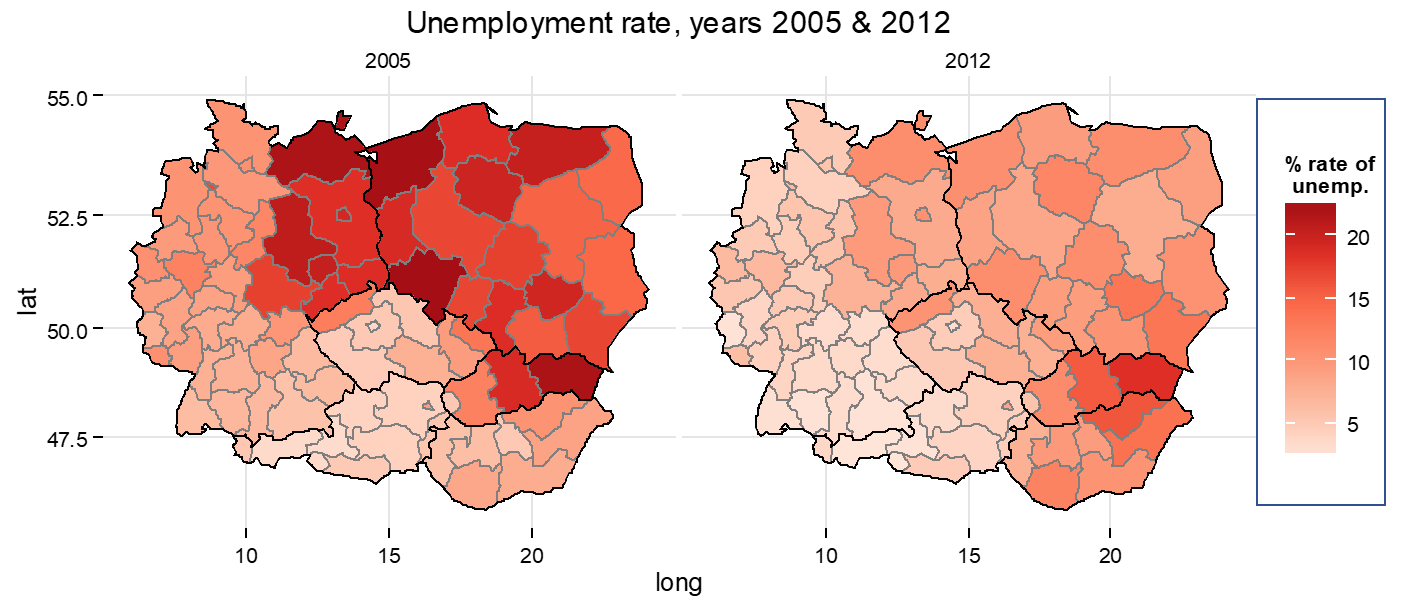
\includegraphics[width=.9\textwidth]{IMG/sp_auto2.PNG}
\end{figure}
\end{frame}
%---------------------------------------------------------------------
\begin{frame}{Introduction - spatial analysis}
Methods of quantitative spatial analysis:\\
\bigskip
\begin{itemize}
    \item Visualization \\Maps, graphical display
    \bigskip
    \item Data exploration \& descriptive methods \\Tools to broadly look at spatial patterns
    \bigskip
    \item Econometric modeling \\Fitting models, testing hypotheses, formalizing spatial dependence, discerning spatial effects from other factor (e.g. macroeconomic)
\end{itemize}
\end{frame}
%---------------------------------------------------------------------
\begin{frame}{Introduction - spatial analysis}
 What are spatial data?\\
\bigskip
\begin{itemize}
    \item Data that are location speciffic and that vary in space.
    \medskip
    \item Referenced by a spatial location $\bm{s}$ (usually 2D),  \\$\bm{s} = (x; y)$; $x$ is longitude (easting) and $y$ is latitude (northing). \\ \medskip
    May also be referenced by a zip code, county or state ID.
    \medskip
    \item Data that are close together in space (time) are often more alike than those that are far apart.
    \medskip
    \item Tobler's first law of geography: \\ ``Everything is related to everything else, but near things are more related than distant things.''
\end{itemize}
\end{frame}
%---------------------------------------------------------------------
\begin{frame}{History of spatial analysis: 1854 -- London -- cholera}
\vspace{-0.5cm}
\begin{figure}
	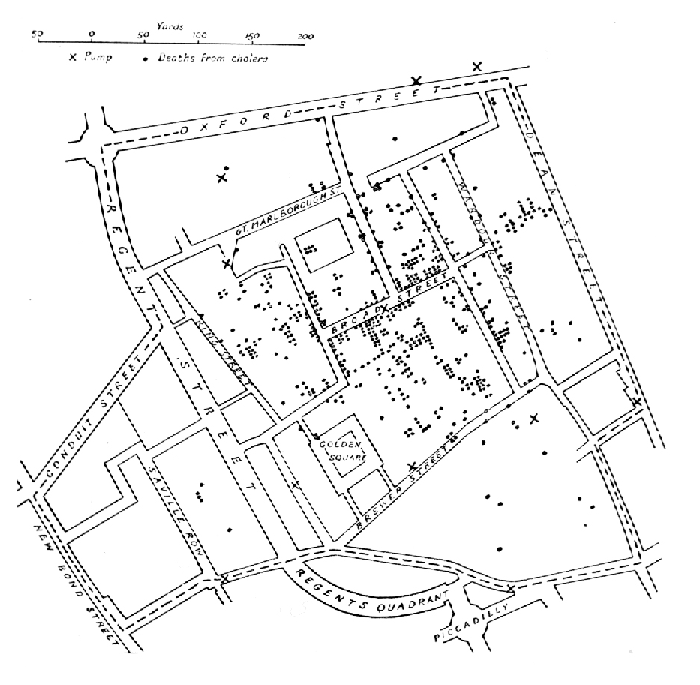
\includegraphics[width=.65\textwidth]{IMG/sp_cholera.eps}
\end{figure}
\end{frame}
%---------------------------------------------------------------------
\begin{frame}{History of spatial analysis: 1854 -- London -- cholera}
 Dr. John Snow: Early spatial analysis\\
\medskip
\begin{itemize}
    \item In August 1854, there was a major Cholera outbreak in the Soho neighbourhood of London, UK. There were 127 cholera related deaths around the area.
    \smallskip
    \item At the time, germ theory (microorganisms causing disease) was not generally accepted. Dr. J. Snow was a MD, pioneer of germ theory and a statistician.
    \smallskip
    \item Dr. John Snow spoke to local residents and mapped where cholera cases occurred. As a result of his map, he was able to pinpoint the public water pump on Broad Street as the source of contaminated water causing the cholera outbreak.
    \smallskip
    \item Dr. Snow used statistics to find a relationship between water sources and cholera cases and subsequently found out that the waterworks company supplying water to Broad Street pump was taking water from a sewage polluted area of the Thames river.
\end{itemize}
\end{frame}
%---------------------------------------------------------------------
\begin{frame}{History of spatial analysis: 1935 -- field experiments}
\vspace{-0.5cm}
\begin{figure}
	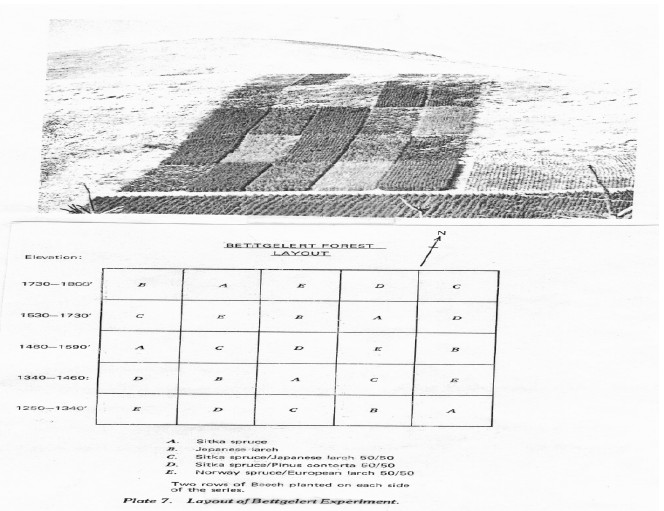
\includegraphics[width=.8\textwidth]{IMG/sp_Fisher.jpg}
\end{figure}
\end{frame}
%---------------------------------------------------------------------
\begin{frame}{History of spatial analysis: 1935 -- field experiments}
 R.A. Fisher: Early spatial analysis\\
\medskip
\begin{itemize}
    \item R.A. Fisher was probably the first to recognize implications of spatial dependency for statistical analysis.
    \smallskip
    \item In his work on design of experiments in agricultural science, he wrote (Fisher, 1935, p. 66):\\
    ``After choosing the area we usually have no guidance beyond the widely verified fact that patches in close proximity are commonly more alike, as judged by the yield of crops, than those which are further apart.''
    \smallskip
    \item Observed spatial variability, i.e. field-to-field variability, was largely due to physical properties of the soil and environmental properties of the field. He avoided the confounding of treatment effects with plot effect with the introduction of randomization.
    \smallskip
    \item Fisher's solution was to eliminate spatial dependency bias by localizing the crops under scrutiny into randomly assigned blocks.
\end{itemize}
\end{frame}
%---------------------------------------------------------------------
\section{Spatial stochastic processes}
\begin{frame}{Spatial stochastic processes}
\end{frame}
%---------------------------------------------------------------------
\begin{frame}{Measuring spatial variables}
Spatial data: measurements and measurement scales
\begin{itemize}
    \item \textbf{Generally, data vary continuously over space, but are measured only at discrete locations.} 
    \begin{itemize}
        \item To characterize spatial variables, spatial aggregation is necessary.
        \item Aggregation of spatial variables may be just another source of bias and potential data mis-manipulation\\ 
        Summary values are influenced by shape and scale of spatial units.\\
        Shape (administrative boundaries) may change over time.
    \end{itemize}
    \item Scale, consistency and relevance should be carefully considered
when collecting and analyzing spatial data
\end{itemize}
\medskip
Spatio-temporal data:
\begin{itemize}
    \item Data that are location specific and repeated in time.
    \item Each variable-observation has a location, time and value.
    \item Similar methods for analysis, with an added time dimension \\(choice of sampling frequency, spatial panel data analysis)
\end{itemize}
\end{frame}
%---------------------------------------------------------------------
\begin{frame}{Measuring spatial distances}
Distances ($d$) can be defined in a variety of ways, yet the following technical conditions should always apply (invariant to spatial translation, i.e. ``shift''):\\
\medskip
\begin{enumerate} 
\item[1] $d(\bm{s}_i, \bm{s}_j) = d(\bm{s}_j, \bm{s}_i)$ \\ \smallskip (symmetry) 
\medskip
\item[2] $d(\bm{s}_i, \bm{s}_i) = 0$  \\ \smallskip (dist. between a point and itself is zero) 
\medskip
\item[3] $d(\bm{s}_i, \bm{s}_j) \leq d(\bm{s}_i) + d(\bm{s}_j)$  \\ \smallskip (triangle inequality; 
$d(\bm{s}_i)$ is the distance from origin) 
\end{enumerate}
\end{frame}
%---------------------------------------------------------------------
\begin{frame}{Measuring spatial distances}
\small{\textbf{Euclidean distances}, measured between two point in the ``ordinary'' Euclidean space. In 2D, the Euclidean distance ($L_2$ norm) is defined as 
$$
d(\bm{s}_i, \bm{s}_j) = \sqrt[]{(s_{ix}-s_{jx})^2+(s_{iy}-s_{jy})^2}\,,
$$
where the $x$ and $y$ subscripts handle planar coordinates. For smaller distances, the computational simplicity is attractive.\\
\medskip
\textbf{Great circle distances} - for larger distances, planar projection accumulates non-negligible errors. The shortest path between two points on a sphere (given their longitudes and latitudes): 
$$
d(\bm{s}_i, \bm{s}_j) = 2r \, \arcsin \,
 \sqrt{ \sin^2 \left( \frac{\phi_j-\phi_i}{2} \right)
       + \cos(\phi_i) \cos(\phi_j)
       \sin^2 \left( \frac{l_j-l_i}{2} \right) }\,,
$$
where $r$ is the radius of the sphere, $\phi_1$ and $\phi_2$ are the latitudes of $\bm{s}_i$ and $\bm{s}_j$ in radians, $l_i$ and $l_j$ are the longitudes (in radians). Its only an approximation when applied to the Earth, which is not a perfect sphere (correct within a 0.5\%; alternative: Vicenty's formulae).\\
\medskip
\textbf{Manhatan distances} - $L_1$ norm, a function on a fixed grid.
}
\end{frame}
%---------------------------------------------------------------------
\begin{frame}{Spatial stochastic processes}
For a generic location $\bm{s}$ given by a vector of $d$ coordinates in a $d$-dimensional Euclidean space, spatial stochastic process \\(``random field'') is often denoted as
$$ Z(\bm{s}): \bm{s} \in D \subseteq \mathbb{R}^d \, .$$
\vspace{-0.5cm}
\begin{itemize}
    \item Typically, $d=2$ for most economic and econometric applications, $d=3$ is often used in fields such as geology or astronomy. 
    \smallskip
    \item $D$ is a fixed finite set of $N$ spatial locations $\bm{s}_1, \bm{s}_2, \dots, \bm{s}_N$. 
    \smallskip
    \item Individual $\bm{s}_i$ units are points in space (say, with GPS-based latitude and longitude coordinates). Sometimes, such points can be associated with non-zero surface area elements.
    \item Much like in time-series analysis, the individual realizations of a spatial stochastic process -- random field -- are often denoted \\$z(\bm{s}_i)$ or, simply, $z_i$.
\end{itemize}
\end{frame}
%---------------------------------------------------------------------
\begin{frame}{Spatial stochastic processes}
Stationarity is a common assumption: a spatial process under scrutiny repeats itself over the domain $D$. If we translate the entire set of coordinates by $\bm{h}$ -- a specific distance in a specified direction, the stochastic process and its features remain unchanged.\\
\medskip
\textbf{Strong stationarity} of a random filed: We start with a finite-dimensional distribution: 
$$F_{\bm{s}_1, \dots,\bm{s}_m }(z_1,\dots, z_m) = P[Z(\bm{s}_1) \leq z_1, Z(\bm{s}_2) \leq z_2, \dots, Z(\bm{s}_m) \leq z_m] \, .$$  
Strong stationarity $\leftrightarrow$~$F$ is invariant under spatial translation $\bm{h}$. Unlike $d_{ij}$ (Euclidean distance between two spatial units $\bm{s}_i$ and $\bm{s}_j$), \\$\bm{h}$ is an orientated distance ``shift'' (spatial translation) vector. \\For strong stationarity:
\begin{equation*}
\begin{aligned}
& P \left[Z(\bm{s}_1) \leq z_1, Z(\bm{s}_2) \leq z_2, \dots, Z(\bm{s}_m) \leq z_m \right] \\
& = P \left[Z(\bm{s}_1+\bm{h}) \leq z_1, Z(\bm{s}_2+\bm{h}) \leq z_2, \dots, Z(\bm{s}_m+\bm{h}) \leq z_m \right] \, .
\end{aligned} 
\end{equation*}
\end{frame}
%---------------------------------------------------------------------
\begin{frame}{Spatial stochastic processes}
\vspace{-0.2cm}
\textbf{Weak  stationarity} (also called second order stationarity) assumes that the first two moments exist, are invariant (and finite) and covariance only depends on spatial translation (orientated distance) $\bm{h}$:
\begin{equation*}
\begin{aligned}  
E[Z(\bm{s})] &= \mu \,, \\
\textnormal{var}[Z(\bm{s})] & = \sigma^2 \,, \\
\textnormal{cov} [Z(\bm{s}+\bm{h}),Z(\bm{s})] = C(\bm{s}+\bm{h}, \bm{s}) & = C(\bm{h}) \,.
\end{aligned} 
\end{equation*}
As autocovariance is a function of $\bm{h}$ only (under weak st.), \\for any spatial points $\bm{s}_i$ and $\bm{s}_j$ such that $\bm{s}_i -\bm{s}_j = \bm{h}$, we can write: 
\begin{equation*}
\textnormal{cov} \left[ Z(\bm{s}_i), Z(\bm{s}_j) \right] = C(\bm{s}_i - \bm{s}_j) = C(\bm{h}) \,.  
\end{equation*}
Covariogram $C(\bm{h})$ is the covariance between two spatial units, separated by $\bm{h}$. For $\bm{h} = \bm{0}$, it simply describes variance: 
$$\textnormal{cov}\,[Z(\bm{s}+\bm{0}),Z(\bm{s})] =  C(\bm{0}) = \textnormal{var}\,[Z(\bm{s})]\,.$$
Under weak dependency, covariance disappears with growing distance: 
$$C(\bm{h}) \rightarrow 0~\textnormal{as}~||\bm{h}|| \rightarrow \bm{\infty}$$.
\end{frame}
%---------------------------------------------------------------------
\begin{frame}{Spatial stochastic processes}
\textbf{Intrinsic stationarity} is less restrictive than weak (second order) stationarity and it is defined in terms of first differences. \\
\smallskip
A spatial process is intrinsically stationary if the difference between two observed spatial points is weakly stationary: 
\begin{equation*} 
\begin{aligned}  
E[Z(\bm{s}+\bm{h})-Z(\bm{s})] &= 0 \,, \\
\textnormal{var}[Z(\bm{s}+\bm{h})-Z(\bm{s})] & = 2\gamma(\bm{h}) \,,
\end{aligned} 
\end{equation*}
where $2\gamma(\bm{h}) \geq 0$ is the variogram. Generally, $2\gamma(\bm{h})$ increases with growing oriented distance $\bm{h}$. \\
\smallskip
The two types of relaxed stationarity are related: weak stationarity implies intrinsic stationarity but not vice versa. For weakly stationary spatial processes (where $E(Z(\bm{s}+\bm{h}))=E(Z(\bm{s}))=\mu$) the variogram simplifies to: 
\begin{equation*}
2\gamma(\bm{h}) = E \left[ \left( Z(\bm{s}+\bm{h}) - Z(\bm{s})  \right)^2 \right],
\end{equation*}
i.e. to the expected squared difference between two observed realizations of a spatial stochastic process. 
\end{frame}
%---------------------------------------------------------------------
\begin{frame}{Spatial stochastic processes}
\textbf{Semivariogram} is denoted as $\gamma(\bm{h})$ and it equals to half the variogram. \\ \smallskip Since  $2\gamma(\bm{h})$ is calculated as expectation of a square, $\gamma(\bm{h}) \geq 0$ for both weakly and intrinsically stationary random fields. \\ \smallskip Also, at $\bm{h}=\bm{0}$, $\gamma(\bm{0}) = 0$ because 
$$ E \left[ \left( Z(\bm{s}_i) - Z(\bm{s}_i)  \right)^2 \right]=0 \textnormal{~for~} \forall \, i\,.$$
Variogram (semivariogram) is a generalization of the covariogram $C(\bm{h})$ and under weak stationarity, the two functions are related by: 
\begin{equation*}
    \gamma(\bm{h}) = C(\bm{0}) - C(\bm{h})\,.
\end{equation*}
If a stationary stochastic process has no spatial dependency at all \\(i.e. $C(\bm{h})=0$ for $\bm{h}\not =\bm{0}$), the semivariogram is constant: $\gamma(\bm{h}) = \textnormal{var}[Z(\bm{s})]$ everywhere, except for $\bm{h}=\bm{0}$, where $\gamma(\bm{0})=0$. 
\end{frame}
%---------------------------------------------------------------------
\begin{frame}{Spatial stochastic processes}
\textbf{Isotropic spatial process} may be defined through a semivariogram:\\  $$\gamma(\bm{h})=\gamma(||\bm{h}||)=\gamma(d).$$ 
Isotropy means that the semivariogram depends only on the distance $d$ between two points and not on direction.\\ \medskip The lack of isotropy -- anisotropy -- means the semivariogram depends on direction as well as distance. \\ \medskip To assess and test anisotropy, we can estimate and plot directional semivariograms (shown next).
\end{frame}
%---------------------------------------------------------------------
\begin{frame}{Spatial stochastic processes}
\textbf{Empirical semivariogram} \\
To perform empirical analysis of distance-based data correlations, we construct the so called empirical semivariogram. First, we divide the distances observed over the domain $D$ into $K$ conveniently chosen intervals: 
$$I_1 = (0, d_1 ], \, I_2 = (d_1, d_2 ], \, \dots \, , \, I_K = (d_{K-1}, d_K ] \, .$$
Here, $d_1$ is the maximum distance within the $I_1$ interval and $d_K$ is the maximum distance observed over the field of data. \\ \smallskip The intervals can be proportional in terms of distance or in terms of sets of observation pairs allocated to each interval (to adjust for unevenly spaced observations). \\ \smallskip Note that distances are determined by $d$ (distance magnitudes) only -- here, we do not use the orientated distances $\bm{h}$.
\end{frame}
%---------------------------------------------------------------------
\begin{frame}{Spatial stochastic processes}
\textbf{Empirical semivariogram} is calculated using the following formula:
\begin{equation*}
\hat{\gamma}(d_k) = 
\frac{1}{2N(d_k)} \sum_{N(d_k)}[Z(\bm{s}_i)-Z(\bm{s}_j)]^2 \,,
\end{equation*}
where $N(d_k)$ is the number of distinct observation pairs in the interval $I_k$ and $\hat{\gamma}(d_k)$ is the semivariogram estimate for its corresponding group (interval) of distances. \\
\bigskip
Usually, we fit a convenient parametric function (exponential, spherical, Gaussian, etc.) to the estimated $\hat{\gamma}(d_k)$ values (shown next). \\ 
\bigskip
The main goal of empirical semivariogram construction is to estimate and visualize the spatial autocorrelation structure of the observed stochastic process.
\end{frame}
%---------------------------------------------------------------------
\begin{frame}{Empirical semivariogram}
\begin{figure}
	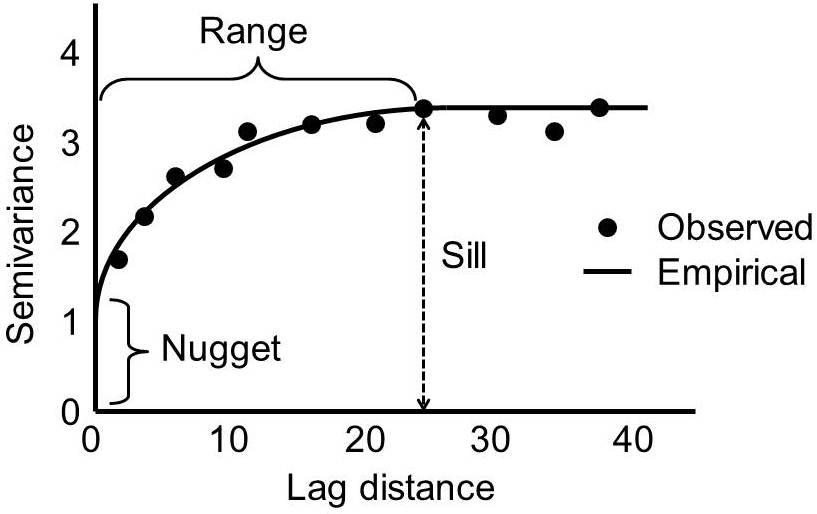
\includegraphics[width=.9\textwidth]{IMG/sp_svgm.jpg}
\end{figure}
\end{frame}
%---------------------------------------------------------------------
\begin{frame}{Empirical semivariogram}
Three main features of an estimated empirical semivariogram: 
\begin{itemize}
\item \textit{Nugget} (nugget effect) describes the micro-scale variations or measurement errors in data. Theoretically, at zero distance, $\gamma(0)=0$. However, two factors play a role here: First, $\gamma(d_1)$ is estimated over the $N(d_1)$ set of pairs, i.e. for the first interval where $ d_{ij} \in (0, d_1 ]$. Second, fitting the empirical semivariogram curve to observed values often causes the non-zero nugget.
\smallskip
\item \textit{Sill} amounts to $\lim_{d \to \infty} \gamma(d)$. The sill corresponds to variance of the stochastic field at distances where spatial dependency (which reduces $\gamma(d)$) no longer applies. $\lim_{d \to \infty} \gamma(d) = C(\bm{0}) = \textit{var}[Z(\bm{s})]$.
\smallskip
\item \textit{Range} is the spatial distance (if any) beyond which the data are not autocorrelated. In a way, range describes the strength of spatial structure -- based on where the semivariogram ``reaches'' its asymptote (sill).
\end{itemize}
\end{frame}
%---------------------------------------------------------------------
\begin{frame}{Empirical semivariogram (fitting)}
\vspace{-0.25cm}
\begin{figure}
	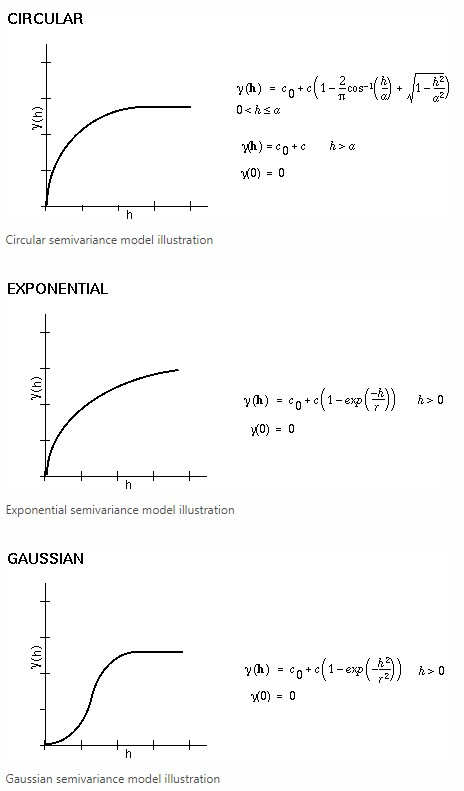
\includegraphics[width=.4\textwidth]{IMG/sp_svgm2.jpg}
\end{figure}
\end{frame}
%---------------------------------------------------------------------
\begin{frame}{Empirical semivariogram (directional semivariogram)}
\begin{figure}
	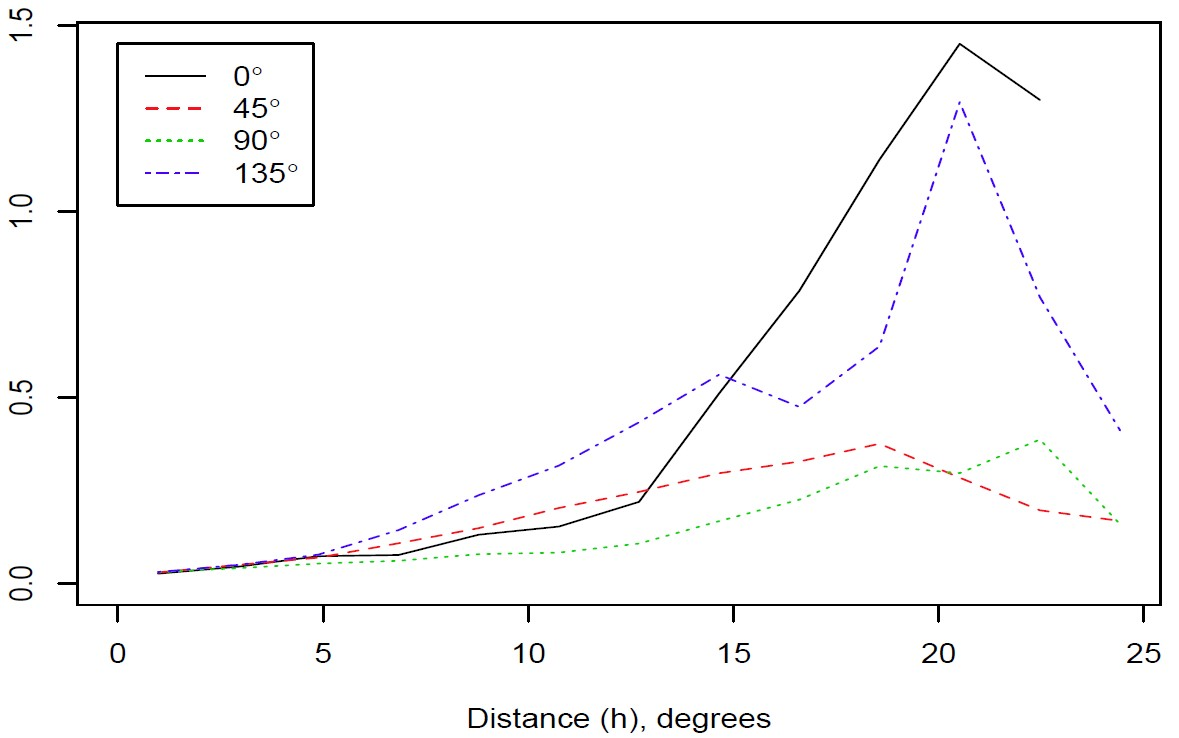
\includegraphics[width=.8\textwidth]{IMG/sp_svgm3.jpg}
\end{figure}
\end{frame}
%---------------------------------------------------------------------
\begin{frame}{Spatio-temporal stochastic processes}
The above discussion can be generalized to accommodate processes that are observed repeatedly over time. \\ \medskip 
Such observations usually exhibit both spatial and temporal dependency and variability.\\ \medskip  
Given the frequency and density limitations of empirical measurements in continuous space and time, we model our observations as realizations of a spatio-temporal random function (random field)
\begin{equation*} 
Z(\bm{s},t), \hspace{1cm} \textnormal{where~} (\bm{s},t) \in \, \mathbb{R}^d \! \times \mathbb{R} \,,
\end{equation*}
the spatio-temporal domain is indexed in space by $\bm{s} \in \mathbb{R}^d$ and in time by $t \in \mathbb{R}$. \\ \medskip 
The separation between spatial and time dimensions is substantial, which is reflected in the notation.
\end{frame}
%---------------------------------------------------------------------
\begin{frame}{Spatio-temporal stochastic processes}
Weak and intrinsic stationarity concepts can be easily expanded from spatial to spatio-temporal data. \\ \medskip
For an intrinsically stationary process $Z(\bm{s},t)$, spatio-temporal semivariograms (STSV) is:
\begin{equation*} 
\gamma(\bm{h};t) = \frac{1}{2} \textnormal{var} \left[ Z(\bm{s}_0+\bm{h} \, ; \> t_0 + t) - Z(\bm{s}_0;t_0) \right],
\hspace{1cm} (\bm{h},t) \in \, \mathbb{R}^d \! \times \mathbb{R}.
\end{equation*}
STSV does not depend on the selection of origin $(\bm{s}_0, t_0) \in \mathbb{R}^d \! \times \mathbb{R}$ (under intrinsic stationarity). \\ \medskip Also, for intrinsically stationary random fields $Z(\bm{s},t)$, the STSV $\gamma(\bm{h};t)$ is non-negative and $\gamma(\bm{0};0) = 0$.
\end{frame}
%---------------------------------------------------------------------
\begin{frame}{Empirical STSV (EU's Unemp., NUTS0, 2002---2016)}
\begin{figure}
	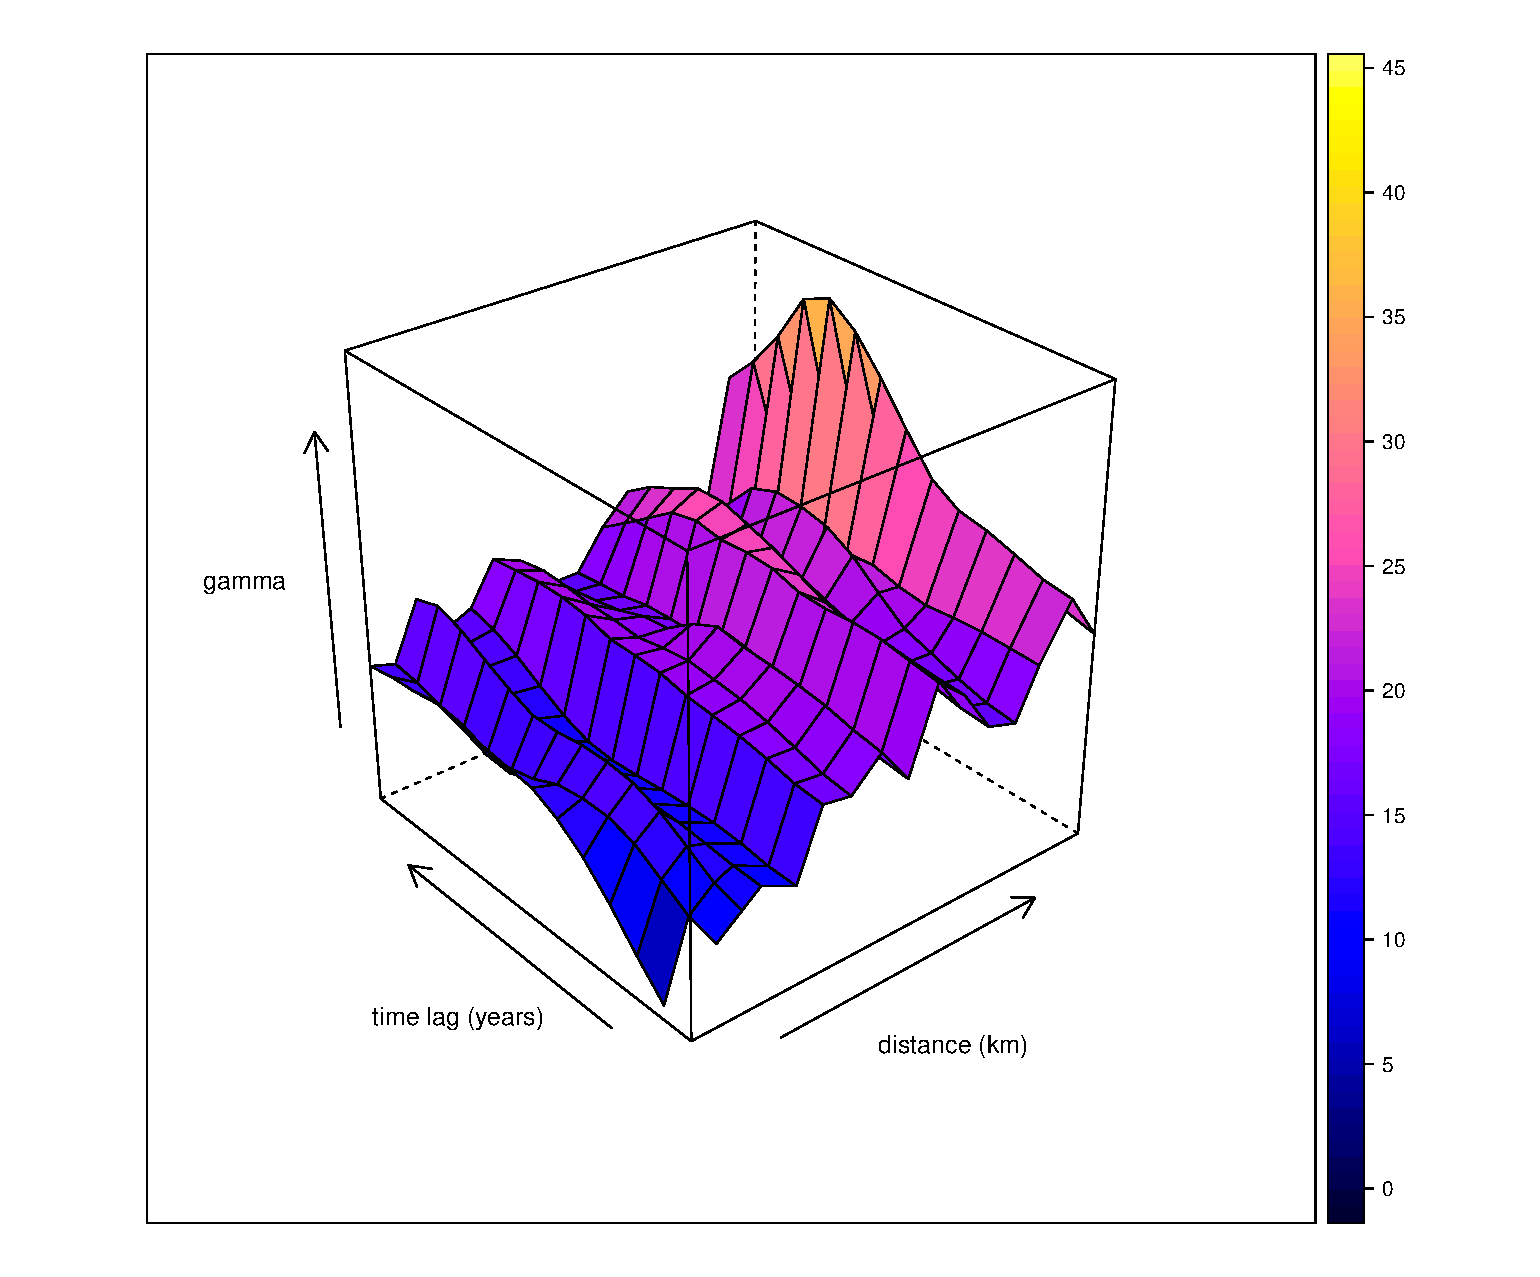
\includegraphics[width=.7\textwidth]{IMG/sp_STV.eps}
\end{figure}
\end{frame}
%---------------------------------------------------------------------
\section{Data exploration \& descriptive methods}
\begin{frame}{Data exploration \& descriptive methods}
\end{frame}
%---------------------------------------------------------------------
\subsection{Interpolation and Krigging}
\begin{frame}{Interpolation}
\textbf{Inverse distance weighting (IDW):} a deterministic method of interpolation with a known scattered set of points. \\ \smallskip Assigned values to unknown points are calculated with a weighted average of the values available at the known points.
\\ \smallskip 
To find an interpolated value $x_0$ at a given point $\bm{s}_0$ based on samples $x_i=x(\bm{s}_i)$ with $i=1,2,\dots,N$ we use a IDW interpolating function:
$$
x(\bm{s}_0) = 
\begin{cases}
    \frac{\sum_{i=1}^N w_i(\bm{s_0})x_i}{\sum_{i=1}^N w_i(\bm{s_0})}, & 
    \textnormal{if~} d(\bm{s}_0,\bm{s}_i) \neq 0 \textnormal{~for all~}i\\
    x_i & \textnormal{if~} d(\bm{s}_0,\bm{s}_i)=0 \textnormal{~for some~}i \, 
\end{cases} 
$$
where $w_i(\bm{s}_0)=\frac{1}{d(\bm{s}_0,\bm{s}_i)^p}\,$, $\bm{s}_0$ is an interpolating (known) point, $d$ is a distance, and $p$ is a positive \textit{real} number (power parameter). \\ \smallskip
Weight decreases as distance increases from the interpolated points. High $p$ assigns greater influence to closest values -- result may turn into a mosaic of tiles (a Voronoi diagram). 
\end{frame}
%---------------------------------------------------------------------
\begin{frame}{IDW interpolation -- illustration}
\begin{figure}
	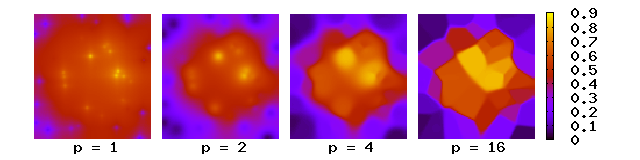
\includegraphics[width=.7\textwidth]{IMG/sp_idw.png}
\end{figure}
\end{frame}
%---------------------------------------------------------------------
\begin{frame}{Krigging}
\begin{itemize}
    \item developed by Daniel G. Krige (1919-2013) \\(originally called ``weighted moving averages'' method) 
    \smallskip
    \item Also known as BLUP (best linear unbiased prediction) and closely related to OLS estimation.
    \smallskip
    \item Returns observed values at sampling locations.
    \smallskip
    \item Interpolates values using the intensity and shape of the empirical (semi)variogram. Results depend on the choice of fitting model \\(Gaussian, spherical, exponential, etc.).
    \smallskip
    \item Uses neighborhood and/or distance search radius.
    \smallskip
    \item Provides standard errors of interpolated values.
    \smallskip
    \item Multiple approaches and generalizations exist (Block Krigging). \\
    \url{http://desktop.arcgis.com/en/arcmap/10.3/tools/3d-analyst-toolbox/how-kriging-works.htm}
\end{itemize}
\end{frame}
%---------------------------------------------------------------------
\begin{frame}{Krigging}
\textbf{Kriging}\\ \medskip
\begin{itemize}
    \item $x(\bm{s}_0)= \sum_{i=1}^N \lambda_i \, x(\bm{s}_i)$ ~~s.t.~~ $\sum_{i=1}^N \lambda_i = 1$. 
    \bigskip
    \item In IDW, $\lambda_i$ depend only on distance to the prediction location.\\
    \bigskip
    \item  With krigging, $\lambda_i$ depend on a fitted model to the measured points, the distance to the prediction location, and the spatial relationships among the measured values around the prediction location (basically, krigging weights follow from the estimated empirical semivariogram: see illustration on the next page).
\end{itemize}
\end{frame}
%---------------------------------------------------------------------
\begin{frame}{Krigging -- illustration}
\begin{figure}
	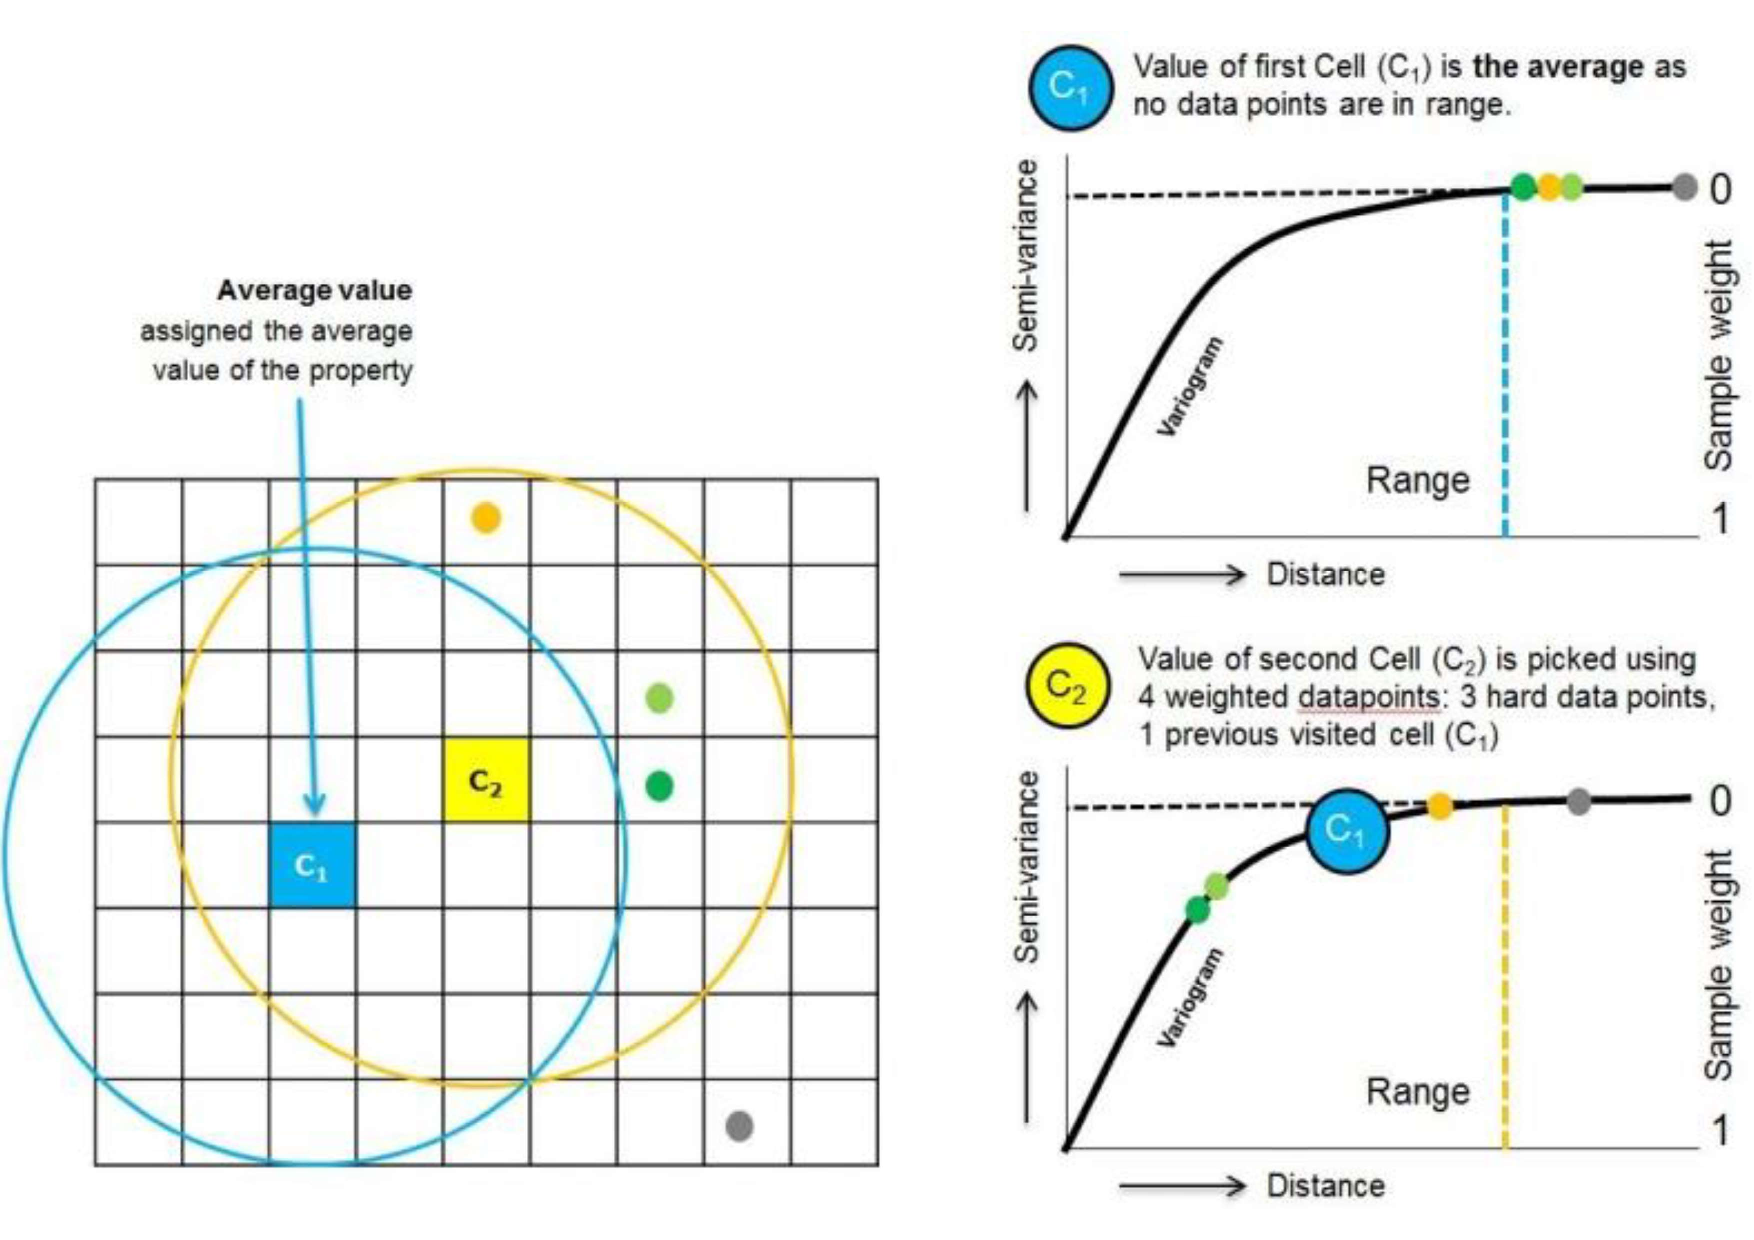
\includegraphics[width=.8\textwidth]{IMG/sp_Krigg.pdf}
\end{figure}
\end{frame}
%---------------------------------------------------------------------
\begin{frame}{Krigging}
\textbf{Ordinary kriging} assumes constant unknown mean only over the search neighborhood of $\bm{s}_{0}$. \\ \medskip
\begin{itemize}
    \item Matrix form: $x(\bm{s}_0)= \bm{\lambda}^{\prime} \, \bm{x}$ ~~s.t.~~ $\bm{\lambda}^{\prime} \bm{1} = 1$. \\
    where $\bm{\lambda}^{\prime} = (\lambda_1,\dots,\lambda_N)$ and $\bm{1}$ is a vector of ones.
    \medskip
    \item Krigging -- solve:~~~~ $\min E(x(\bm{s}_0 - \bm{\lambda}^{\prime} \, \bm{x})^2$ s.t. $\bm{\lambda}^{\prime} \bm{1} = 1$.\\
    \medskip
    \item  Minimum variance of $x(\bm{s}_0)$: $~\sigma^2= \sum_{i=1}^N \lambda_i \gamma (\bm{s}_i,\,\bm{s}_0)~+~m \,$
    \medskip
    \item is obtained when $\sum_{i=1}^N \lambda_i \gamma (\bm{s}_i,\,\bm{s}_j)~+~m = \gamma (\bm{s}_j,\,\bm{s}_0)$ for all $j$. \\
    \medskip
    Here, $\gamma$ is the semivarogram, $m$ is an additional LM parameter (mean estimate) that ensures unbiasedness of the estimate. \\For additional discussion and alternative estimation methods \\(simple, universal krigging, etc.), see\\
    \url{https://en.wikipedia.org/wiki/Kriging}
\end{itemize}
\end{frame}
%---------------------------------------------------------------------
\subsection{Definition of neighbors}
\begin{frame}{Definition of neighbors}
\begin{itemize}
    \item Fotheringham et al (2002): ``Spatial dependency is the extent to which the value of an attribute in one location depends on the values of the attribute in nearby locations.''
    \medskip
    \item Different definitions of spatial dependency are possible.
    \medskip
    \item To discuss spatial dependency, spatial autocorrelation, corresponding tests and spatial econometric models, we need to formalize the concept of \textbf{nearby locations -- neighbors}
\end{itemize}
\end{frame}
%---------------------------------------------------------------------
\begin{frame}{Definition of neighbors}
\begin{itemize}
	\item \textbf{Distance-based approach} defines two units as neighbors if their distance does not exceed some ad-hoc predefined threshold: $\tau$. \\
	\medskip
	\begin{itemize}
		\item Can generate ``islands'' (units with zero neighbors), if $\tau$ is low compared to minimum distances among unit pairs.
		\smallskip
		\item Less suited for analysis of areas with uneven geographic density (of measurements). 
	\end{itemize}
	\medskip
	\item \textbf{Centroids} are used for measuring distances between units with non-zero areas (e.g. regions)\\
	\medskip
	\begin{itemize}
		\item Centroids can be purely geographical, ``main'' city locations, population-weighted, transportation-weighted (highway/railway), etc.
	\end{itemize}
\end{itemize}
\end{frame}
%---------------------------------------------------------------------
\begin{frame}{Definition of neighbors}
\begin{figure}
	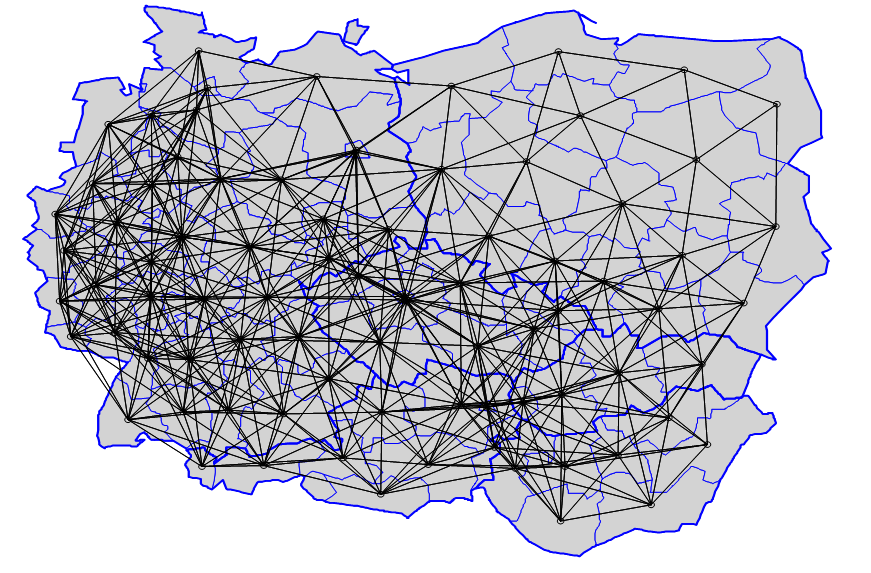
\includegraphics[width=.7\textwidth]{IMG/sp_neigb.PNG}
	\caption[]{Plot for distance-based neighbors (NUTS2), maximum neighbor distance threshold at 250 km}
\end{figure}
\end{frame}
%---------------------------------------------------------------------
\begin{frame}{Definition of neighbors}
\begin{itemize}
\item \textbf{Contiguity-based approach} spatial units (regions) are neighbors if they share a common border (at least one point).
\bigskip 
\item \textbf{Generalized contiguity approach} is based on the premise that a ``second order'' neighbor is the neighbor of a first order neighbor (the actual contiguous neighbor). \\ \smallskip With this type of approach, we can define a maximum neighborhood lag (order) to control for the highest accepted number
of neighbors traversed (not permitting cycles).	
\end{itemize}
\end{frame}
%---------------------------------------------------------------------
\begin{frame}{Definition of neighbors}
\textbf{$\bm{k}$ Nearest neighbors ($\bm{k}$NN)} \\
\medskip
For each spatial unit, we search for a preset number of $k$ nearest units that we define as its neighbors. 
\medskip
\begin{itemize}
	\item Solves for differences in areal densities ($k$ neighbors are ensured for each unit).
	\smallskip
	\item Usually leads to asymmetric spatial connectivity matrices with potentially flawed neighborhood interpretation. 
	\smallskip
	\item Illustration for $k = 3$   (neighbors only shown for 2 units):
	\begin{figure}
		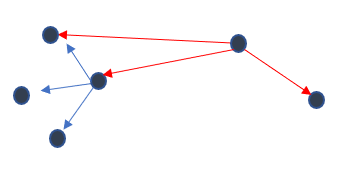
\includegraphics[width=.2\textwidth]{IMG/sp_neigb2.PNG}
	\end{figure}
\end{itemize}
\end{frame}
%---------------------------------------------------------------------
%\subsection{Spatial connectivity and weights matrices}
\begin{frame}{Spatial connectivity matrix ($\bm{C}$)}
$$
~~\bm{C} = \begin{bmatrix}
0 & 1 & 1 & 1 \\
1 & 0 & 1 & 0 \\
1 & 1 & 0 & 1 \\
1 & 0 & 1 & 0
\end{bmatrix}\quad \text{~~a 4-unit example}$$
$$c_{ij}=
	\begin{cases}
	1 & \text{if $i$ and $j$ are neighbors,}\\
	0 & \text{if $i$ and $j$ are not neighbors.}
	\end{cases}$$
\begin{itemize}
	\item Zeros on the diagonal -- units are not neighbors to themselves.
	\smallskip
	\item Spatial connectivity matrix interpretation: 
	\smallskip
	\begin{itemize}
		\item row/column 1: unit 1 is neigbor to units 2,3,4
		\item row/column 2: unit 2 is neigbor to units 1,3 (not 4)
	\end{itemize}
	\smallskip
    \item Matrix $\bm{C}$ is symmetric (for $k$NN, transformations are available).
\end{itemize}
\end{frame}
%---------------------------------------------------------------------
\begin{frame}{Spatial weights matrix ($\bm{W}$)}
\vspace{-0.5cm}
$$
\bm{C} = \begin{bmatrix}
0 & 1 & 1 & 1 \\
1 & 0 & 1 & 0 \\
1 & 1 & 0 & 1 \\
1 & 0 & 1 & 0
\end{bmatrix}\rightarrow 
\bm{W}=
\begin{bmatrix}
0 & \tfrac{1}{3} & \tfrac{1}{3} & \tfrac{1}{3} \\[2pt]
\tfrac{1}{2} & 0 & \tfrac{1}{2} & 0 \\[2pt]
\tfrac{1}{3} & \tfrac{1}{3} & 0 & \tfrac{1}{3} \\[2pt]
\tfrac{1}{2} & 0 & \tfrac{1}{2} & 0
\end{bmatrix}
$$
\begin{itemize}
	\item Usually, $\bm{W}$ is row-standadrized (to unity): 
	$w_{ij} = \frac{c_{ij}}{\sum^N_{j=1} c_{ij}}$.
	\smallskip
	\item Binary (connectivity) indicators $c_{ij}$ may be generalized prior to standardization. Hence, instead of binary $c_{ij}$, we may use inverse distances (linear, squared, \dots) -- given assumed decay in spatial dependency over distance. \\ \medskip Validity of any such prior information (decay pattern) will influence subsequent analysis (spatial dependency tests, spatial regression models).
\end{itemize}
\end{frame}
%---------------------------------------------------------------------
\begin{frame}{Spatial weights matrix ($\bm{W}$)}
\vspace{-0.2cm}
$$
\bm{W}=
\begin{bmatrix}
0 & \tfrac{1}{3} & \tfrac{1}{3} & \tfrac{1}{3} \\[2pt]
\tfrac{1}{2} & 0 & \tfrac{1}{2} & 0 \\[2pt]
\tfrac{1}{3} & \tfrac{1}{3} & 0 & \tfrac{1}{3} \\[2pt]
\tfrac{1}{2} & 0 & \tfrac{1}{2} & 0
\end{bmatrix}
$$
\begin{itemize}
	\item Each row of $\bm{W}$ ``provides'' weights for an expected value of an observed spatial variable $y_i$ -- weighted averages (fitted values) can be calculated as $\hat{\bm{y}} = \bm{Wy}$. For example:
	\begin{align*}
	\hat{y}_1 & =  \tfrac{1}{3} y_2 + \tfrac{1}{3} y_3 + \tfrac{1}{3} y_4 \\
	&\dots \\
	\hat{y}_4 & = \tfrac{1}{2} y_1  + \tfrac{1}{3} y_3 
	\end{align*}
	\item Observed values of variables can be used to predict corresponding values for neighboring spatial units.
	\smallskip
	\item In this context, $\hat{y}_i$ is often called \textit{spatial lag} of $y_i$.
\end{itemize}
\end{frame}
%---------------------------------------------------------------------
\begin{frame}{Definition of neighbors}
\vspace{-0.3cm}
\begin{figure}
	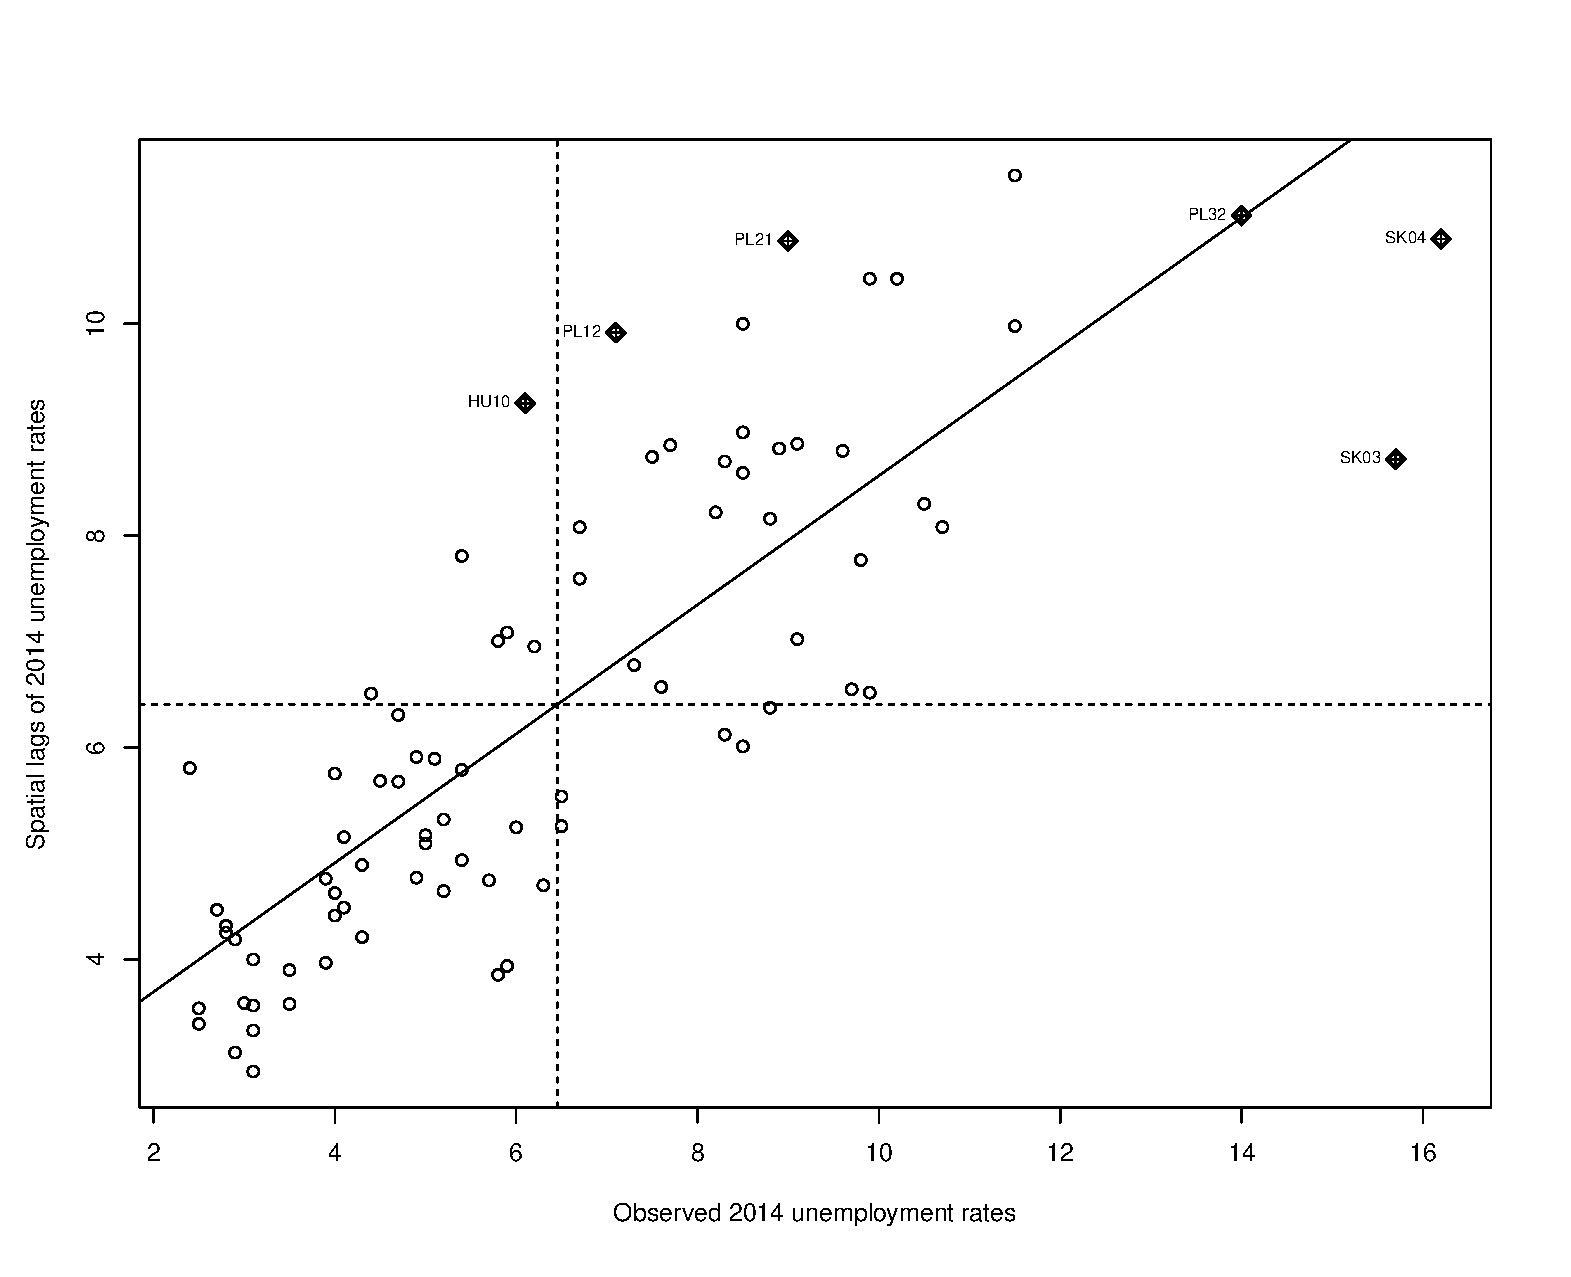
\includegraphics[width=.7\textwidth]{IMG/sp_MoranPlot.eps}
	\caption[]{Moran plot for unemployment rate, 2014, NUTS2 (AT, CZ, DE, HU, PL, SK): observed values vs. spatial lags.}
\end{figure}
\end{frame}
%---------------------------------------------------------------------
\begin{frame}{Sample selection in spatial data analysis}
\begin{itemize}
    \item Spatially autocorrelated processes are defined in terms of individual units and their interactions with neighbors. 
    \smallskip
    \item Clearly, we can only assess the impact of neighboring units if such units are part of our sample. Hence, in spatial econometrics, we usually do not draw limited samples from a particular area.
    \smallskip
    \item Instead, we work with data from adjacent units located in unbroken (``complete'') study areas.  
    \smallskip
    \item Otherwise, $\bm{C}$ and $\bm{W}$ matrices would be misleading and we could not consistently estimate spatial interactions and effects.
    \smallskip    
    \item Generally speaking, spatial analysis should include the whole geographically defined area/region instead of using random sampling (from a ``population'' of regions within the relevant area). 
\end{itemize}
\end{frame}
%---------------------------------------------------------------------
\subsection{Spatial dependency tests}
\begin{frame}{Spatial dependency tests}
\begin{itemize}
    \item Positive spatial autocorrelation occurs if high or low values \\of a variable cluster in space. 
    \medskip
    \item For negative spatial autocorrelation, spatial units tend to be surrounded by neighbors with very dissimilar observations. 
    \medskip
    \item Spatially random data lack any spatial pattern.
    \medskip
    \item Sometimes, spatial dependency patterns are easy to discern visually using choropleths. 
    \medskip
    \item However, a formal approach towards evaluation of spatial dependency is often required.
\end{itemize}
\end{frame}
%---------------------------------------------------------------------
\begin{frame}{Moran's $I$}
Measure of global spatial autocorrelation, overall clustering of data:
\begin{equation*}
I = \frac{N}{W}\,\bm{z}'\bm{Wz}(\bm{z}'\bm{z})^{-1},
\end{equation*}     
where 
\begin{itemize}
    \item[] $N$ is the number of spatial observations (units) of the variable under scrutiny (say, $\bm{y}$),
    \smallskip
    \item[] $\bm{z}$ is the centered form of $\bm{y}$: $z_i = y_i - \bar{y}$.\\
    (Note a recast: $y_i = \beta_0 + z_i$. If SLRM is expanded by regressors, Moran's $I$ can be applied to regression residuals).
    \smallskip
    \item[] The standardization factor $W = \sum_{i}\sum_{j}w_{ij}$ corresponds to the sum of all elements of the spatial weights matrix $\bm{W}$. \\For row-standardized $\bm{W}$ matrices, $\tfrac{N}{W}=1$. Moran's $I$ can be used with $\bm{C}$ matrices (binary, generalized) as well.
\end{itemize}
\end{frame}
%---------------------------------------------------------------------
\begin{frame}{Moran's $I$}
\vspace{-0.2cm}
\begin{equation*}
I = \frac{N}{W}\,\bm{z}'\bm{Wz}(\bm{z}'\bm{z})^{-1},
\end{equation*}     
In most empirical circumstances, $I \in [ -1,1 ]$. Under the null hypothesis of spatial randomness, Moran’s $I$ is asymptotically normally distributed with the following first two moments:
\begin{equation*}
E(I) = -\frac{1}{N-1} \hspace{0.5cm} 
\textnormal{and} \hspace{0.5cm} 
\textnormal{var}(I) = \frac{N^2W_1 - NW_2 +3W^2}{(N^2-1)W^2} \,,
\end{equation*}  
where $W_1 = \sum_i \sum_j (w_{ij}+w_{ji})^2$ and $W_2 = \sum_i (\sum_j w_{ij} + \sum_j w_{ji})^2$.\\
\medskip
Normality assumption $\rightarrow$ calculate a $z$-score 
$$z=\frac{I-E(I)}{\sqrt{\textnormal{var}(I)}} $$\\
and test for statistical significance of Moran's $I$: whether neighboring units are more similar $(I > E(I))$ or more dissimilar $(I < E(I))$ than they would be under the null hypothesis of spatial randomness.
\end{frame}
%---------------------------------------------------------------------
\begin{frame}{Local Moran's $I$}
\begin{itemize}
    \item Moran's $I$ yields only one statistic that summarizes the nature of spatial dependency in the observed variable -- it assumes geographical homogeneity (stationarity) in the data. 
    \smallskip
    \item If such assumption does not hold (spatial dependency varies over space), then Moran's $I$ test loses power and the ``global'' statistic is non-descriptive. 
    \smallskip
    \item To address this problem, we can use Local Moran's $I$ statistic \\(for row-standardized $\bm{W}$):
    \begin{equation*}
    I_i = \frac{z_iN}{\bm{z}'\bm{z}}\bm{w}_{i}\bm{z} \, .
    \end{equation*}    
    \item The expected value of  Local Moran's $I$ under the null hypothesis of no spatial autocorrelation is: $E(I_i)=-w_i/(N-1)$. Here, $w_i$ is the sum of elements in the $i$-th row of $\bm{W}$.
\end{itemize}
\end{frame}
%---------------------------------------------------------------------
\begin{frame}{Local Moran's $I$}
    \begin{equation*}
    I_i = \frac{z_iN}{\bm{z}'\bm{z}}\bm{w}_{i}\bm{z} \, .
    \end{equation*}    
\begin{itemize}
    \item Values of $I_i > E(I_i)$ indicate positive spatial autocorrelation, i.e. that the $i$-th region is surrounded by regions that, on average, are similar to the $i$-th region with respect to the observed variable $y$. 
    \item $I_i < E(I_i)$ would suggest negative spatial autocorrelation.
    \item Significance of spatial dependency is then evaluated using $var(I_i)$ and the corresponding $z$-score.
    \bigskip
    \item We may see the global nature of Moran's $I$ from
    \begin{equation*} 
    I = \frac{1}{N}\sum_{i=1}^N I_{i} \,.
    \end{equation*}   
\end{itemize}
\end{frame}
%---------------------------------------------------------------------
\begin{frame}{Geary's $C$}
 Variance test similar (in principle) to the Durbin-Watson test statistic for residuals' autocorrelation in time-series regressions.
 \begin{equation*}
C = \frac{N-1}{2W}\,
    \frac{\sum_{i}\sum_{j}w_{ij}(y_i-y_j)^2}
         {\sum_{i}(y_i-\bar{y})^2} \,,
\end{equation*}   
where all elements follow from previous slides. Empirical Geary's $C$ values range from 0 to 2. However, occurrences of $C>2$ are possible.\\
\smallskip
\begin{itemize}
    \item Under the null of no spatial autocorrelation, first two moments are:
\begin{equation*}
E(C) = 1\, ,\hspace{0.5cm}
\textnormal{var}(C) = \frac{(N-1)(2W_1 + W_2) - 4W^2 }{2(N+1)W^2} \,,
\end{equation*}  
\item Positive spatial dependency: $C < 1$.\\ Negative spatial autocorrelation is reflected in $C > 1$.
\smallskip
\item $z$-transformation is asymptotically normally distributed. Therefore, $z(C)$ can be used for testing spatial randomness.
\end{itemize}
\end{frame}
%---------------------------------------------------------------------
\subsection{Clusters -- hotspots and coldspots}
\begin{frame}{Clusters -- hotspots and coldspots}
Getis' $G^{\ast}$: spatial clusters and hotspot analysis\\
\smallskip
\begin{itemize}
    \item Clustering analysis by Getis can only be performed for positively autocorrelated spatial data.
    \smallskip
    \item $G_i^{\ast}(\tau) = \frac{\sum_{j=1}^N c_{ij}^{\ast} y_j}{\sum_{j=1}^N y_j} \,,$\\
    \smallskip
    where $c_{ij}^{\ast}$ come from amended distance-based (arbitrary $\tau$ used) connectivity matrix $\bm{C}^{\ast} = \bm{C}+\bm{I}_N$; i.e. $y_i$ observations enter $G_i^{\ast}(\tau)$ calculation. Observations of $y$ are assumed to have a natural origin and positive support.
    \smallskip
    \item $G_i^{\ast}(\tau)$ is a local stastic, a proportion of the aggregated $y_j$ values that lie within $\tau$ of $i$ to the total sum of $y_j$ observations.
    \smallskip
    \item Alternatively, Getis' statistic is calculated using $\bm{C}$ (not $\bm{C}^{\ast}$) and denoted $G_i(\tau)$ 
\end{itemize}
\end{frame}
%---------------------------------------------------------------------
\begin{frame}{Clusters -- hotspots and coldspots}
\begin{itemize}
    \item If we observe high values of $y_j$ within distance $\tau$ of unit $i$, then $G_i^{\ast}(\tau)$ would be relatively high compared to its expected value under the null hypothesis of full spatial randomness: $$E \left[G_i^{\ast}(\tau) \right] = \frac{c_i^{\ast}}{N}\,,$$ where $c_i^{\ast}$ is the sum of elements of $i$-th row of $\bm{C}^{\ast}$.
    \medskip 
    \item Also, under the $H_0$ of spatial randomness, we can write
    $$
    \textnormal{var} \left[G_i^*(\tau) \right] = 
    \frac{c_i^*(N-c_i^*)}{N^2 (N-1)}
    \left( \frac{Y_{i2}^*}{(Y_{i1}^*)^2} \right) , 
    $$ 
    where $Y_{i1}^*=\tfrac{\sum_j y_j}{N}$ and $Y_{i2}^*=\tfrac{\sum_j y_j^2}{N}-(Y_{i1}^*)^2$.
    \medskip 
    \item High positive $z$-score indicates ``hotspot'' (cluster of high values) and vice versa. Critical values provided by Getis and Ord. \\Say, for $N = 100$ and $\alpha = 5\%$, the $z$-scores would have to exceed $\pm 3.289$ for a statistically significant hot/cold spot.
\end{itemize}
\end{frame}
%---------------------------------------------------------------------
\begin{frame}{Clusters -- hotspots and coldspots}
\begin{figure}
	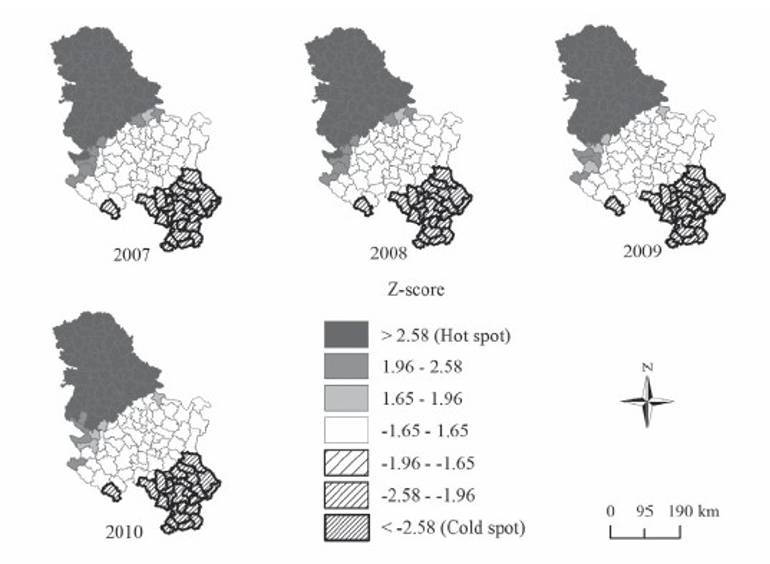
\includegraphics[width=.7\textwidth]{IMG/sp_coldspot.PNG}
	\caption{Spatial clusters (hot and cold spots) of the municipalities in Serbia by the level of average monthly net earning from 2001 to 2010}
\end{figure}
\end{frame}
%---------------------------------------------------------------------
\section{Spatial regression models (parametric)}
\begin{frame}{Spatial regression models}
\end{frame}
%---------------------------------------------------------------------
\begin{frame}{Spatial regression models}
\begin{itemize}
\item Spatial regression models allow us to discern the influence of geographic factors (spatial autocorrelation, spill-over effects) from other relevant factors/variables -- say, economic -- that may be subject to macroeconomic policy tools.
\medskip
\item Observed data are characterized (indexed) by geographic location, distances between geo-coded units play a crucial role.
\end{itemize}
\end{frame}
%---------------------------------------------------------------------
\begin{frame}{Spatial regression models}
\textbf{Spatial regression models -- examples}
\medskip
\begin{itemize}
	\item House prices depend on utility-related variables (area in m$^2$, number of rooms/bedrooms, elevator, etc.). At the same time, prices in a given area/neighborhood tend to be correlated -- usually, positive spatial autocorrelation is present. 
	\smallskip
	\item Highway gas-stations' revenues depend on distance from \\a capital/major city (traffic intensities may be measured -- or proxied by distances). \\Can be considered as a special case of one-dimensional spatial dependency (distance measured along the highway route). 
	\smallskip
	\item Increased policing activity in a given area (county) may decrease local crime levels while causing increased illegal activities in nearby counties -- a negative spatial autocorrelation example.
	\smallskip
	\item Macroeconomic shocks (both positive and negative) may spill more prominently among spatially close economies: we need to account for such effects in econometric models.
	\end{itemize}
\end{frame}
%---------------------------------------------------------------------
\begin{frame}{Spatial regression models}
\textbf{Spatial regression models -- discussion}
\medskip
\begin{itemize}
	\item Great proportion of spatial effects (spatial dependencies) is closely related to missing variables (significant yet often non-measurable) for a regression model.
	\smallskip
	\item Spatial lag is a proxy variable for (potentially many) unobservable factors. For example, using EU's labor market and/unemployment regression models:
	\smallskip
	\begin{itemize}
		\item Work commuting among regions/districts/states and the problematic consistent measurements of this phenomenon.
		\smallskip
		\item Language, qualification and administrative barriers on labor market.
		\smallskip
		\item Aerial distances vs. topology and transportation infrastructure.
	\end{itemize}
	\smallskip
	\item Spatial models may provide a simple and interpretable tool for analysis of macroeconomic (regional) dynamics.
\end{itemize}
\end{frame}
%---------------------------------------------------------------------
\begin{frame}{Spatial regression models -- main motivations}
\vspace{-0.2cm}
\begin{itemize}
\item \textit{Omitted variables} motivation: discussed on previous slide.
\smallskip
\item \textit{Time-dependency}: agents make decisions influenced by the behavior of other agents in previous periods (state authorities may set taxes that reflect policy actions taken by their neighbors in previous periods).
\smallskip
\item \textit{Spatial heterogeneity} motivation is largely based on panel data methods and regression models. Spatially close units exhibit more similar individual effects as compared to non-neighboring units. 
\smallskip
\item \textit{Externalities-based} motivation comes from a well-established economic concept: individuals and regions may be subject to positive/negative consequences of activities exercised by unrelated third parties (heavy traffic, air pollution, etc.).
\smallskip
\item \textit{Model uncertainty} motivation: spatial autocorrelation may be used in circumstances where we face uncertainty in terms of specifying a proper data generating process (DGP). 
\end{itemize} 
Note that motivations are not mutually exclusive.
\end{frame}
%---------------------------------------------------------------------
\begin{frame}{Spatial regression models}
Generalized nesting spatial (GNS) model 
\begin{equation*}
\begin{aligned}
  \bm{y} &= \lambda \bm{W\!y} + \alpha \bm{\iota} + \bm{X \beta} + \bm{W\!X\theta} + \bm{u} \,, \\
  \bm{u} &= \rho \bm{W\!u} + \bm{\varepsilon} \,,
\end{aligned}
\end{equation*}
where $\bm{W\!y}$ is the spatial lag, $\bm{W\!X}$ is the spatial lag for regressor matrix $\bm{X}$ and $\bm{W\!u}$ describes spatial interactions (spatial lag) among disturbance elements. Elements $\lambda$, $\rho$ and $\bm{\theta}$ are the spatial parameters, estimated along with $\alpha$ and $\bm{\beta}$.\\ \bigskip
Under the null hypothesis of no spatial dependency \\($\lambda = \rho =0$  and $\bm{\theta}=\bm{0}$), GNS simplifies to 
\begin{equation*}
  \bm{y} = 
  \alpha \bm{\iota} + \bm{X \beta} + \bm{\varepsilon} \,,
\end{equation*}
Using apropriate null restrictions, GNS may be transformed to different types of spatial models.
\end{frame}
%---------------------------------------------------------------------
\begin{frame}{Spatial regression models}
\begin{figure}
	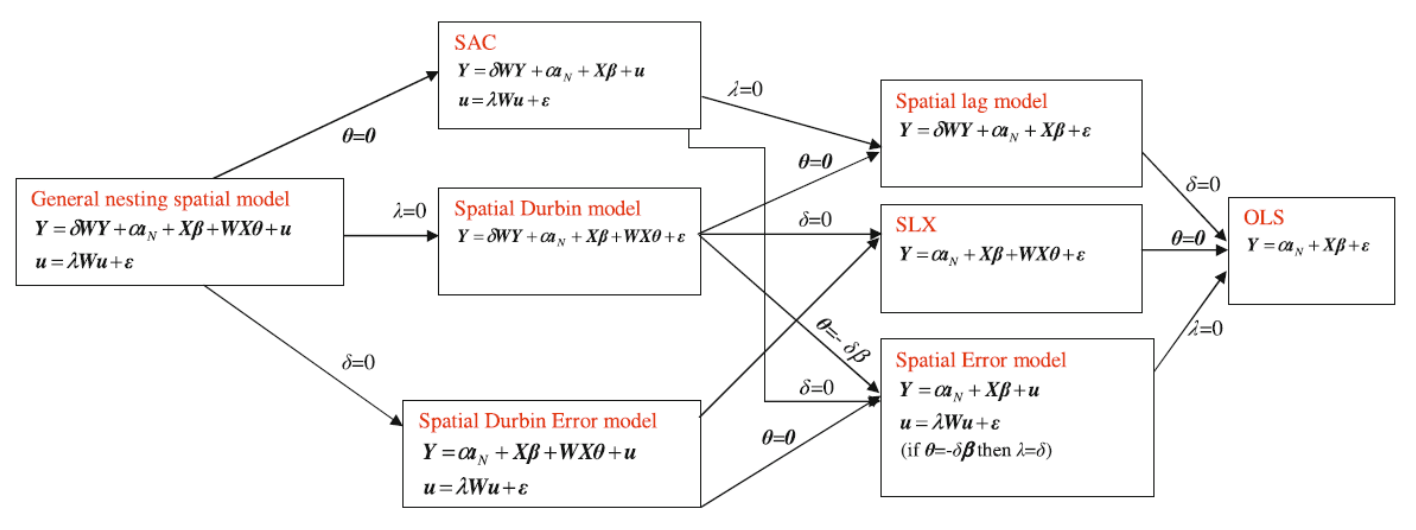
\includegraphics[width=1\textwidth]{IMG/sp_reg.PNG}
	\caption{The relationship between different spatial dependence models for cross-sectional data (source: Elhorst, 2014). Note: this illustration is based on a slightly modified notation of spatial parameters.}
\end{figure}
\end{frame}
%---------------------------------------------------------------------
\begin{frame}{Spatial lag model}
By assuming spatial interactions in the dependent variable only, \\($\bm{\theta}=\bm{0}$ and $\rho=0$), we simplify GNS into a spatial lag model (SLM):
\begin{equation*} 
\bm{y} = \lambda \bm{W\!y} + \alpha \bm{\iota} + \bm{X \beta} + \bm{\varepsilon}\,.
\end{equation*}
The SLM specification is used commonly throughout empirical literature, e.g. in models describing taxes imposed by governments. Reduced form of SLM can be expressed as:
\begin{equation*} 
(\bm{I}_{N} - \lambda \bm{W}) \bm{y} = \alpha \bm{\iota} + \bm{X \beta} + \bm{\varepsilon}\,,
\end{equation*}
where $\bm{I}_{N}$ is an $(N\! \times \!N)$ identity matrix and the RHS regression coefficients explain the variability of individual $y_{i}$ observations that is not explained spatially. Also, if the inverse to $(\bm{I}_{N} - \lambda \bm{W})$ exists, we can express DGP for $\bm{y}$ as
\begin{equation*}
\bm{y} = (\bm{I}_{N} - \lambda \bm{W})^{-1} (\alpha \bm{\iota} + \bm{X \beta} + \bm{\varepsilon})\,.
\end{equation*}
\end{frame}
%---------------------------------------------------------------------
\begin{frame}{Spatial lag model}
\begin{equation*} 
\bm{y} = \lambda \bm{W\!y} + \alpha \bm{\iota} + \bm{X \beta} + \bm{\varepsilon}\,.
\end{equation*}
\begin{itemize}
    \item For each $y_i$, the element $\textit{SpatialLag}(y_{i}) = \bm{w}_i \bm{y}$ enters the equation, where $\bm{w}_i$ is the $i$-th row of $\bm{W}$.
    \smallskip
    \item For model stability, we assume $\lambda \in (-1,1)$. \\(rule of thumb, see Elhorst, 2014, Spatial Econometrics; From Cross-Sectional Data to Spatial Panels and the discussion provided next).
    \smallskip
    \item Coefficients $\bm{\beta},~\alpha$ and $\lambda$ are estimated by MLE (if distributional assumptions -- e.g. normality of the error term -- can be made).  Otherwise, GMM may be applied.
    \smallskip
    \item Coefficients $\bm{\beta}^{\prime} = (\beta_1, \dots, \beta_k)$ explain (ceteris paribus) variability in $\bm{y}$ that is not explained spatially.
\end{itemize}
\end{frame}
%---------------------------------------------------------------------
\begin{frame}{Spatial Durbin model}
If we drop the simplifying assumption $\bm{\theta}=\bm{0}$ from SLM, we get the spatial Durbin model (SDM):
\begin{equation*} 
  \bm{y} = \lambda \bm{W\!y} + \alpha \bm{\iota} + \bm{X \beta} + \bm{W\!X\theta} + \bm{\varepsilon}\,.
\end{equation*}
For example, if $y_i$ describes household income in a region $i$, then such income is influenced by incomes (say, wages) in neighboring regions and by both ``domestic'' and neighboring rates of unemployment, labor force productivities, etc.  
\\ \medskip
By analogy to the SLM case -- and  given $(\bm{I}_{N} - \lambda \bm{W})^{-1}$ exists -- we may write the DGP as follows:
\begin{equation*}
\bm{y} = (\bm{I}_{N} - \lambda \bm{W})^{-1} (\alpha \bm{\iota} + \bm{X \beta} + \bm{W\!X\theta}+ \bm{\varepsilon})\,.
\end{equation*}
\end{frame}
%---------------------------------------------------------------------
\begin{frame}{Spatial error model}
Spatial error model (SEM) is another frequently used specification of the spatial model. SEM is obtained from the GNS model by assuming $\lambda=0$ and $\bm{\theta}=\bm{0}$. Hence, spatial interactions take place only among the error terms: 
\begin{equation*}
\begin{aligned}
\bm{y} = \alpha \bm{\iota} + \bm{X \beta} + \bm{u}\,, \\
 \bm{u} = \rho \bm{W\!u} + \bm{\varepsilon}\,.
\end{aligned}
\end{equation*}
Theoretical (macroeconomic) reasoning of the spatial dependency is not required for SEMs -- this approach can be used to model a situation where endogenous variables are influenced by exogenous factors that are omitted from the main equation and spatially autocorrelated. Alternatively, unobserved shocks may follow spatial pattern(s).
\end{frame}
%---------------------------------------------------------------------
\begin{frame}{Spatial model stability conditions}
\begin{enumerate}
\item Spatial matrix $\bm{C}$ is a non-negative matrix of known constants with zeros on the diagonal (if this holds for $\bm{C}$, it holds for the row-standardized $\bm{W}$ as well).
\smallskip
\item Spatial weak dependency  holds. Two alternative conditions: (a) The row and column sums of $\bm{C}$ should be uniformly bounded in absolute value as $N$ (the number of observed units) goes to infinity. (b) The row and column sums of $\bm{C}$ should not diverge to infinity at a speed equal to or faster than the growth of sample size $N$. Condition (b) is more general (relaxed) and (a) is its special case.
\smallskip
\item Matrices $(\bm{I}_{N} - \lambda \bm{W})$ and $(\bm{I}_{N} - \rho \bm{W})$ are non-singular. If the underlying $\bm{C}$ matrix is symmetric and non-negative, this condition is satisfied whenever $\lambda$ and $\rho$ lie within the $(1/\kappa_{min}, 1)$ interval, where $\kappa_{min}$ denotes the smallest (most negative) real eigenvalue of $\bm{W}$ and 1 is the largest eigenvalue for a row-standardized $\bm{W}\!.$ \vspace{0.2cm} \\
\end{enumerate}    
\end{frame}
%---------------------------------------------------------------------
\begin{frame}{ML estimation of SLMs and SDMs}
\begin{itemize}
    \item The RHS regressor element $\bm{W\!y}$ in SLM or SDM is correlated with the error term. Hence, OLS estimation of models with spatially lagged endogenous variables is biased and inconsistent.
    \smallskip 
    \item ML estimators for such models are consistent (other methods are possible: GMM, 2SLS).
    \smallskip
    \item We use a slightly modified SDM notation to describe ML estimator for both SLMs and SDMs, as their likelihood functions coincide (SLM is a special case of SDM, with $\bm{\theta}=\bm{0}$ imposed). 
    \smallskip
    \item First, we expand the DGP of SDM by $\textit{iid}$ normality assumption for residuals: 
    \begin{equation*} 
    \begin{aligned}
    \bm{y} &= (\bm{I}_{N} - \lambda \bm{W})^{-1} (\alpha \bm{\iota} + \bm{X \beta} + \bm{W\!X\theta}+ \bm{\varepsilon})\,, \\ 
    \bm{\varepsilon} &\sim N(\bm{0}, \sigma_{\varepsilon}^2 \, \bm{I}_{N}) \,,
    \end{aligned}
    \end{equation*}
    where $\sigma_{\varepsilon}^2$ is the variance of $\bm{\varepsilon}$.
\end{itemize}
\end{frame}
%---------------------------------------------------------------------
\begin{frame}{ML estimation of SLMs and SDMs}
\begin{itemize}
    \item In $\bm{y} = (\bm{I}_{N} - \lambda \bm{W})^{-1} (\alpha \bm{\iota} + \bm{X \beta} + \bm{W\!X\theta}+ \bm{\varepsilon})\,,$ we use substitution $\bm{Z}=[\bm{\iota} \,, \bm{X} \,, \bm{W\!X}]$ and $\bm{\delta}= \left[ \alpha \,, \bm{\beta} \,, \bm{\theta} \right]^{'}$. 
    \smallskip
    \item We can re-arrange DGP of the SDM/SLM equation as: 
    \begin{equation*}
    \begin{aligned}
    \bm{y} &= (\bm{I}_{N} - \lambda \bm{W})^{-1} \bm{Z \delta} \, + \,
    (\bm{I}_{N} - \lambda \bm{W})^{-1} \bm{\varepsilon}\,, \\ 
    \bm{\varepsilon} &\sim N(\bm{0}, \sigma_{\varepsilon}^2 \, \bm{I}_{N})\,.
    \end{aligned}
    \end{equation*}
    \item The above substitution allows us to use a single likelihood function for both SLM and SDM: for SDMs, we use $\bm{Z}=[\bm{\iota} \,, \bm{X} \,, \bm{W\!X}]$. \\ \smallskip For SLMs, $\bm{Z}=[\bm{\iota} \,, \bm{X}]$ and analogous amendments are made to the vector of parameters $\bm{\delta}$.
    \smallskip
    \item Note how our substitution transforms the original SDM model
    \begin{equation*} 
    \bm{y} = \lambda \bm{W\!y} + \alpha \bm{\iota} + \bm{X \beta} + \bm{W\!X\theta} + \bm{\varepsilon}\,.
    \end{equation*}
    into
    \begin{equation*}
    \bm{y} = \lambda \bm{W\!y} + \bm{Z \delta} + \bm{\varepsilon}\, \qquad \rightarrow \qquad
    \bm{\varepsilon} = \bm{y} - \bm{W\!y} - \bm{Z \delta}.
    \end{equation*}
\end{itemize}
\end{frame}
%---------------------------------------------------------------------
\begin{frame}{ML estimation of SLMs and SDMs}
\begin{itemize}
    \item The log-likelihood function for the SLM (and SDM) model may be outlined as
    \begin{equation*}
    \begin{aligned}
    LL(\lambda,\bm{\delta}, \sigma_{\varepsilon}^2) &= - \frac{N}{2} \log (\pi \sigma_{\varepsilon}^2) +
    \log | \bm{I}_{N} - \lambda \bm{W} | - 
    \frac{\bm{e}^{'} \bm{e} }{2\sigma_{\varepsilon}^2}\,, \\
    \bm{e} &= \bm{y} - \lambda \bm{Wy} - \bm{Z \delta}\,,
    \end{aligned}
    \end{equation*}
    where $N$ is the number of spatial units, $| \bm{I}_{N} - \lambda \bm{W} |$ is the determinant of this $N \! \times \! N$ matrix and $\bm{e}$ is a vector of residuals.
    \smallskip
    \item Direct estimation (maximization) of the $LL$ function is subject to multiple computational issues. Alternative approach -- by means \\of iterating over concentrated log-likelihood functions -- is used.
\end{itemize}
\end{frame}
%---------------------------------------------------------------------
\begin{frame}{ML estimation of SEMs}
\begin{itemize}
    \item We add $\textit{iid}$ normality assumption to $\bm{\varepsilon}$ residuals of the SEM:
    \begin{equation*}
    \begin{aligned}
    \bm{y} &= \bm{X \beta} +  (\bm{I}_{N} - \rho \bm{W})^{-1} \bm{\varepsilon}\,, \\ 
    \bm{\varepsilon} &\sim N(\bm{0}, \sigma_{\varepsilon}^2\,\bm{I}_{N})\,,
    \end{aligned}
    \end{equation*}
    where the intercept term has been incorporated into the $\bm{X \beta}$ expression for simplicity. 
    \smallskip
    \item Now, the log-likelihood function for SEMs has the form
    \begin{equation*}
    \begin{aligned}
    LL(\bm{\beta}, \rho, \sigma_{\varepsilon}^2) &= - \frac{N}{2} \log (\pi \sigma_{\varepsilon}^2) +
    \log | \bm{I}_{N} - \rho \bm{W} | - 
    \frac{\bm{e}^{'} \bm{e} }{2\sigma_{\varepsilon}^2}\,, \\
    \bm{e} &= (\bm{I}_{N} - \rho \bm{W}) (\bm{y} - \bm{X \beta})\,.
    \end{aligned}
    \end{equation*}
    \item Again, for computational reasons, concentrated log-likelihood functions are calculated iteratively to maximize $LL$ function and obtain parameter estimates and corresponding standard errors. 
\end{itemize}
\end{frame}
%---------------------------------------------------------------------
\begin{frame}{ML estimation \& testing of spatial models}
\begin{itemize}
    \item $LL$ functions  for SDMs (SLMs) and SEMs may be amended to accommodate binomial, count, multinomial and other dependent variables (LeSage, Pace: Introduction  to  spatial  econometrics).
    \smallskip
    \item Likelihood ratio ($LR$) test can be used to evaluate spatial model specification through a set of conveniently chosen restrictions leading to two alternative nested models:
\begin{equation*}
\textit{LR} = 2(\mathcal{L}_{ur}-\mathcal{L}_{r}) \,\,\, \underset{H_0}{\sim} \,\,\, \chi_q^2 \, ,
\end{equation*}
where $\mathcal{L}_{ur}$ is the maximized $LL$ function  of the estimated spatial model. The null hypothesis is used to enforce zero restriction on all parameters describing spatial autocorrelation ($\lambda$, $\bm{\theta}$ or $\rho$ -- given specification of the unrestricted model) and $\mathcal{L}_{r}$ is the maximized $LL$ of the non-spatial model.
\smallskip
\item $LR$ tests may be applied more generally (different restrictions may be evaluated).
\end{itemize}
\end{frame}
%---------------------------------------------------------------------
\begin{frame}{SLM vs SEM specification tests}
\begin{itemize}
    \item LM-based test for SEM specification evaluates the null hypothesis of no spatial autocorrelation of residuals against the alternative of SEM specification: 
\begin{equation*}
\textit{LM-SEM}=\frac{1}{T}
\left(\frac{\bm{\hat{u}}^{'}\bm{W\hat{u}}}{\hat{\sigma}^2}\right)^{2} 
\,\,\, \underset{H_0}{\sim} \,\,\, \chi_1^2 \,\,,
\end{equation*}
where $\hat{\sigma}^2$ is the estimated variance of residuals $\bm{\hat{u}}$ and $T=\textnormal{tr}(\bm{W}^{'}\bm{W} \! + \! \bm{W}^2)$ is trace of the matrix. Note that the $\textit{LM-SEM}$ statistic is just a scaled version of Moran's $I$.
\smallskip
\item The $\textit{LM-SEM}$ test is not robust against SLM specification (spatial dependency in $y$).
\end{itemize}
\end{frame}
%---------------------------------------------------------------------
\begin{frame}{SLM vs SEM specification tests}
\begin{itemize}
    \item The $\textit{LM-SLM}$ statistic is used in OLS-estimated linear models to test $H_0$ of spatial independence in $\bm{y}$ against the alternative of its spatial autocorrelation (SLM): 
\begin{equation*} 
\textit{LM-SLM}=\frac{1}{N \, J_{\lambda,\bm{\beta}}}
\left(\frac{\bm{\hat{u}}^{'}\bm{Wy}}{\hat{\sigma}^2}\right)^{2} 
\,\,\, \underset{H_0}{\sim} \,\,\, \chi_1^2 \,\,,
\end{equation*}
where the term $J_{\lambda,\bm{\beta}} = \left[ (\bm{WX\hat{\beta}})^{'}\bm{M}(\bm{WX\hat{\beta}}) + T \hat{\sigma}^2 \right] \! / N \hat{\sigma}^2$ is calculated using the vector of OLS-estimated parameters $\bm{\hat{\beta}}$ and the ``residual maker'' (orthogonal projection matrix) $\bm{M} = \bm{I}_N - \bm{X}(\bm{X}^{'}\bm{X})^{-1}\bm{X}^{'}$.
\smallskip
\item The $\textit{LM-SLM}$ test is not robust against autocorrelated error term (SEM-type).
\end{itemize}
\end{frame}
%---------------------------------------------------------------------
\begin{frame}{SLM vs SEM specification tests}
\begin{itemize}
    \small{
    \item The test for a spatial error process that is robust to local presence of \\a spatial lag is given as:
    \begin{equation*} 
    \textit{RLM-SEM}=\frac{1}{T-T^2(NJ_{\lambda,\bm{\beta}})^{-1}}
    \left(\frac{\bm{\hat{u}}^{'}\bm{W\hat{u}}}{\hat{\sigma}^2}
    -T(NJ_{\lambda,\bm{\beta}})^{-1}
    \frac{\bm{\hat{u}}^{'}\bm{Wy}}{\hat{\sigma}^2}
    \right)^{2} 
    \! \underset{H_0}{\sim} \chi_1^2,
    \end{equation*}
    }% end small
\textnormal{where the subtraction of a correction factor that accounts for the local misspecification (potentially omitted spatial lag process) is visible. 
    \smallskip
    \item By $\textit{RLM-SEM}$, we test the $H_0$ of no spatial dependency in residuals (OLS-estimated) against the alternative of SEM specification, while controlling for possible local spatial lag (SLM process). 
    } % normal
\end{itemize}
\end{frame}
%---------------------------------------------------------------------
\begin{frame}{SLM vs SEM specification tests}
\begin{itemize}
    \item Test for a spatial lag process robust to local presence of spatial error autocorrelation is defined as:
    \begin{equation*}
    \textit{RLM-SLM}=\frac{1}{N \, J_{\lambda,\bm{\beta}} - T}
    \left(\frac{\bm{\hat{u}}^{'}\bm{Wy}}{\hat{\sigma}^2}
    - \frac{\bm{\hat{u}}^{'}\bm{W\hat{u}}}{\hat{\sigma}^2} \right)^{2} 
    \,\,\, \underset{H_0}{\sim} \,\,\, \chi_1^2 \,\,.
    \end{equation*}
    \item Heteroskedasticity-robust versions of statistics $\textit{LM-SEM}$ and $\textit{LM-SLM}$ are available. 
    \smallskip
    \item Heteroskedasticity-robust versions of the $\textit{RLM-SEM}$ and $\textit{RLM-SLM}$ tests are not easily accessible as accounting for heteroskedasticity leads to highly non-linear expressions.
\end{itemize}
\end{frame}
%---------------------------------------------------------------------
\begin{frame}{Marginal effects in spatial models}
\begin{itemize}
	\item In spatial models (SLM, SDM), there are two basic types of marginal effects: direct and indirect effects. \\ \bigskip 
	Sometimes a third effect -- total effect -- is reported: a sum of the previous two effects. 
	\bigskip
	\item In presence of spatial autocorrelation among observed variables (and for SDM), if a given explanatory variable in some $i$-th unit changes, than not only the dependent variable in the $i$-th unit is expected to change (direct effect) but also the dependent variables in other units (neighbors of unit $i$) would change. \\ \bigskip Such effect across spatial units is the indirect effect, sometimes called ``spillover''.
	\end{itemize}
\end{frame}
%---------------------------------------------------------------------
\begin{frame}{Marginal effects in spatial models}
\begin{itemize}
	\item Marginal effects can be conveniently illustrated using a slightly modified GNS model:
\begin{equation*}
\bm{y} = (\bm{I}_N - \lambda \bm{W})^{-1}
         (\bm{X \beta}+\bm{WX\theta}) + \bm{r} \,,
\end{equation*}
where $\bm{r}$ contains both the intercept and (potentially spatially dependent) error term. Marginal effects for some arbitrary regressor $\bm{x}_k$ are given by a Jacobian matrix of first derivatives of the expected values of $\bm{y}$ with respect to the explanatory variable: 
\begin{equation*}
\frac{\partial E(\bm{y})}{\partial \bm{x}_k} = 
\begin{pmatrix}
		\dfrac{ \partial E(\bm{y})}{ \partial x_{1k}} & \cdots & \dfrac{\partial E(\bm{y})}{ \partial x_{Nk}}
	\end{pmatrix} = 	
	\begin{pmatrix}
		\dfrac{\partial E(y_{1})}{\partial x_{1k}} & \cdots & \dfrac{\partial E(y_{1})}{\partial x_{Nk}} \\
		\vdots & \ddots & \vdots \\
		\dfrac{\partial E(y_{N})}{\partial x_{1k}} &\cdots & \dfrac{\partial E(y_{N})}{\partial x_{Nk}} \\
	\end{pmatrix}.
\end{equation*}
\end{itemize}	
\end{frame}
%---------------------------------------------------------------------
\begin{frame}{Marginal effects in spatial models}
\begin{itemize}
	\item After some re-arranging, we can write:
\begin{equation*}
\frac{\partial E(\bm{y})}{\partial \bm{x}_k}
    =(\bm{I}_N-\lambda \bm{W})^{-1} (\bm{I}_N \beta_k + \bm{W} \theta_k)\,.
\end{equation*}
\item 
For convenience and clarity, the RHS may also be re-written as:
\begin{equation*}
\frac{\partial E(\bm{y})}{\partial \bm{x}_k}
    =(\bm{I}_N-\lambda \bm{W})^{-1}
	\begin{pmatrix}
		\beta_{k} & w_{12}\theta_{k}& \cdots & w_{1N}\theta_{k}\\
		w_{21}\theta_{k}& \beta_{k} & \cdots & w_{2N}\theta_{k}\\
		\vdots & \vdots & \ddots & \vdots \\
		w_{N1}\theta_{k} & w_{N2}\theta_{k} & \cdots & \beta_{k} \\
	\end{pmatrix}\,. 
\end{equation*}
\item Recall that $w_{ij}$ denotes element of the $\bm{W}$ matrix and $w_{ij} > 0$ if two spatial units $i$ and $j$ are neighbors (and zero otherwise). \\$\beta_k$ and $\theta_k$ are parameters of the GNS/SDM, corresponding to the $k$-th regressor. The RHS is a $N\!\times\!N$ matrix.
\end{itemize}	
\end{frame}
%---------------------------------------------------------------------
\begin{frame}{Marginal effects in spatial models}
\begin{equation*}
\frac{\partial E(\bm{y})}{\partial \bm{x}_k}
    =(\bm{I}_N - \lambda \bm{W})^{-1}
	\begin{pmatrix}
		\beta_{k} & w_{12}\theta_{k}& \cdots & w_{1N}\theta_{k}\\
		w_{21}\theta_{k}& \beta_{k} & \cdots & w_{2N}\theta_{k}\\
		\vdots & \vdots & \ddots & \vdots \\
		w_{N1}\theta_{k} & w_{N2}\theta_{k} & \cdots & \beta_{k} \\
	\end{pmatrix}\,. 
\end{equation*}
\begin{itemize}
	\item Each diagonal element of the partial derivatives matrix  represents a direct effect and every off-diagonal element represents an indirect effect.
	\smallskip
	\item Direct effects and indirect effects differ across spatial units. Each element of the RHS matrix might be different. 
	\smallskip
	\begin{itemize}
	    \item Individual direct effects differ because the diagonal elements of $(\bm{I}_N - \lambda \bm{W})^{-1}$ are different for each unit (given $\lambda \neq 0$).
	    	\smallskip
	    \item Indirect effects are different because off-diagonal element of both $\bm{W}$ and $(\bm{I}_N - \lambda \bm{W})^{-1}$ are different if $\lambda \neq 0$ and/or $\theta_k \neq 0$.
	\end{itemize} 
\end{itemize}	
\end{frame}
%---------------------------------------------------------------------
\begin{frame}{Marginal effects in spatial models}
\vspace{-0.3cm}
\begin{equation*}
\frac{\partial E(\bm{y})}{\partial \bm{x}_k}
    =(\bm{I}_N - \lambda \bm{W})^{-1}
	\begin{pmatrix}
		\beta_{k} & w_{12}\theta_{k}& \cdots & w_{1N}\theta_{k}\\
		w_{21}\theta_{k}& \beta_{k} & \cdots & w_{2N}\theta_{k}\\
		\vdots & \vdots & \ddots & \vdots \\
		w_{N1}\theta_{k} & w_{N2}\theta_{k} & \cdots & \beta_{k} \\
	\end{pmatrix}\,. 
\end{equation*}
\begin{itemize}
	\item In absence of spatial autocorrelation of $\bm{y}$ and $\bm{x}_k$, i.e. if both $\lambda = 0$ and $\theta_k = 0$, then all off-diagonal elements equal zero. In this case, indirect effects are not present. Also, direct effects are constant (equal to $\beta_k$) across all spatial units as $(\bm{I}_N - \lambda \bm{W})^{-1}$ simplifies to $\bm{I}_N$ if $\lambda=0$. 
	\medskip
    \item The indirect effects that occur if $\theta_k \neq 0$ and $\lambda = 0$ are referred to as \textbf{local effects}. The name arises from the fact that such effect only arise from the neighborhood of a given unit. For example, the effect of $x_{jk}$ ($k$-th regressor for the $j$-th unit) on $y_i$ is nonzero only if units $i$ and $j$ are neighbors (i.e. $w_{ij} > 0$). For non-neighboring units, $x_{jk}$ has no effect on $y_i$.
\end{itemize}	
\end{frame}
%---------------------------------------------------------------------
\begin{frame}{Marginal effects in spatial models}
\begin{equation*}
\frac{\partial E(\bm{y})}{\partial \bm{x}_k}
    =(\bm{I}_N - \lambda \bm{W})^{-1}
	\begin{pmatrix}
		\beta_{k} & w_{12}\theta_{k}& \cdots & w_{1N}\theta_{k}\\
		w_{21}\theta_{k}& \beta_{k} & \cdots & w_{2N}\theta_{k}\\
		\vdots & \vdots & \ddots & \vdots \\
		w_{N1}\theta_{k} & w_{N2}\theta_{k} & \cdots & \beta_{k} \\
	\end{pmatrix}\,. 
\end{equation*}
\begin{itemize}
	\item The indirect effects that occur if $\lambda \neq 0$ and $\theta_k = 0$ are referred to as \textbf{global effects}. The name comes from the fact that effects on $y_i$ originate from units that lie within the neighborhood of $i$ as well as from units outside this neighborhood. Mathematically, this is due to the fact that matrix $(\bm{I}_N-\lambda \bm{W})^{-1}$ does not contain zero elements (given $\lambda \neq 0$) -- even though $\bm{W}$ does contain (usually many) zero elements.
	\medskip
    \item For $\lambda \neq 0$ and $\theta_k \neq 0$, both local and global indirect effect are present and they cannot be separated from each other.
\end{itemize}	
\end{frame}
%---------------------------------------------------------------------
\begin{frame}{Marginal effects in spatial models}
\begin{equation*}
\frac{\partial E(\bm{y})}{\partial \bm{x}_k}
    =(\bm{I}_N - \lambda \bm{W})^{-1}
	\begin{pmatrix}
		\beta_{k} & w_{12}\theta_{k}& \cdots & w_{1N}\theta_{k}\\
		w_{21}\theta_{k}& \beta_{k} & \cdots & w_{2N}\theta_{k}\\
		\vdots & \vdots & \ddots & \vdots \\
		w_{N1}\theta_{k} & w_{N2}\theta_{k} & \cdots & \beta_{k} \\
	\end{pmatrix}\,. 
\end{equation*}
\begin{itemize}
    \item The presence or absence of spatial autocorrelation $\rho$ in the error term of GNS/SDM has no impact on the marginal effects: as we take the first derivative of $E(\bm{y})$ with respect to $\bm{x}_k$, the $\bm{r}= (\alpha \bm{\iota} + \rho \bm{W\!u} + \bm{\varepsilon})$ element disappears because it is a ``constant''.
    \medskip
    \item Considering the complexity of marginal effects for one regressor, the problem of presenting estimation output from a model with multiple regressors may be severe: even if reliable estimates $\hat{\lambda}, \hat{\bm{\beta}}$ and $\hat{\bm{\theta}}$ are available, we have to deal with a $N\!\times\!N$ matrix of marginal (direct and indirect) effects for each regressor.
\end{itemize}	
\end{frame}
%---------------------------------------------------------------------
\begin{frame}{Marginal effects in spatial models}
\begin{equation*}
\frac{\partial E(\bm{y})}{\partial \bm{x}_k}
    =(\bm{I}_N - \lambda \bm{W})^{-1}
	\begin{pmatrix}
		\beta_{k} & w_{12}\theta_{k}& \cdots & w_{1N}\theta_{k}\\
		w_{21}\theta_{k}& \beta_{k} & \cdots & w_{2N}\theta_{k}\\
		\vdots & \vdots & \ddots & \vdots \\
		w_{N1}\theta_{k} & w_{N2}\theta_{k} & \cdots & \beta_{k} \\
	\end{pmatrix}\,. 
\end{equation*}
Estimated marginal effects are usually presented in an aggregated form. For each regressor, we usually report two (sometimes three) statistics:
 \begin{itemize}
    \item Summary indicator for direct effects is calculated as the average of all diagonal elements (of the Jacobian for a given regressor $\bm{x}_k$). 
    \medskip
    \item Indirect effects are reported as the average of all off-diagonal elements. 
    \medskip
    \item The above statistics are usually reported along with their corresponding standard errors and statistical significance indicators ($p$-values) -- see \textcolor{blue}{\underline{\href{http://www.springer.com/cda/content/document/cda_downloaddocument/9783642403392-c2.pdf}{Elhorst (2014)}}} for technical discussion.
\end{itemize}	
\end{frame}
%---------------------------------------------------------------------
\begin{frame}{Marginal effects in spatial models}
\vspace{-0.3cm}
\begin{equation*}
\frac{\partial E(\bm{y})}{\partial \bm{x}_k}
    =(\bm{I}_N - \lambda \bm{W})^{-1}
	\begin{pmatrix}
		\beta_{k} & w_{12}\theta_{k}& \cdots & w_{1N}\theta_{k}\\
		w_{21}\theta_{k}& \beta_{k} & \cdots & w_{2N}\theta_{k}\\
		\vdots & \vdots & \ddots & \vdots \\
		w_{N1}\theta_{k} & w_{N2}\theta_{k} & \cdots & \beta_{k} \\
	\end{pmatrix}\,. 
\end{equation*}
\begin{itemize}
    \item Total effect is just a sum of the direct and indirect impacts. Total standard errors, $z$ scores and significance levels are also calculated by aggregating the underlying direct impacts and spillovers. 
    \smallskip
    \item Motivation: in many empirical applications, the direct and indirect effects may come with opposite signs. Therefore, at some higher level of spatial aggregation, direct impacts and spillovers could cancel out. For example, positive direct effects may come at the ``price'' of equally prominent negative spillovers. 
    \smallskip
    \item Total impacts are often reported along with their direct/indirect constituents -- even if there are no contradicting signs of direct/indirect impacts. 
\end{itemize}	
\end{frame}
%---------------------------------------------------------------------
\begin{frame}{Marginal effects in spatial models}
\begin{itemize}
	\item Sample output from a SLM (model with a single regressor).
	
	\end{itemize}
\begin{table}[]
\centering
\caption{Estimated direct, indirect and total   impacts}
\begin{tabular}{llll}
&         &          &             \\
& Mean    & Std. dev & t-statistic \\
\hline
Direct effect                                                                                          & 0.586   & 0.0148   & 39.6106     \\
Indirect effect                                                                                        & 1.084 & 0.0587   & 18.4745     \\
Total effect                                                                                           & 1.670    & 0.0735   & 22.7302    
\end{tabular}
\end{table}
\end{frame}
%---------------------------------------------------------------------
\begin{frame}{Drawbacks of SLMs/SDMs/SEMs}
\begin{itemize}
\item In SDM/SLM, the ratio between direct and indirect effect for \\a regressor $\bm{x}_k$ is independent of $\beta_k$. This is because the $\beta_k$ coefficients cancel out in the numerator and denominator of such ratio (direct/indirect effects). 
\smallskip
\item This ratio depends only on the parameter $\lambda$ and on the $\bm{W}$ matrix specification. 
\smallskip 
\item Hence, direct/indirect effect ratio is the same for all regressors in \\a given spatial model.
\smallskip
\item Unfortunately, this ``behavior'' (identical relative strengths of direct and indirect effects for all regressors) seems rather implausible in many types of empirical applications.
\end{itemize}
\end{frame}
%---------------------------------------------------------------------
\begin{frame}{Drawbacks of SLMs/SDMs/SEMs}
\begin{itemize}
    \item $\bm{W}$ matrices cannot be estimated along with model parameters. 
    \medskip
    \item Rather, $\bm{W}$ needs to be specified prior to model estimation. 
    \medskip
    \item There is little theoretical background for choosing the ``right'' \\$\bm{W}$ matrix specification. 
    \medskip
    \item As $\bm{W}$ matrix in a SLM/SDM/SEM changes, the estimated parameters tend to change as well. Large changes to $\bm{W}$ may \\cause large changes in estimated parameters.
    \medskip
    \item The variety of available neighborhood definitions and standardization methods implies that researchers usually evaluate several alternative spatial structure settings in order to verify model stability and robustness of the results. 
\end{itemize}
\end{frame}
%---------------------------------------------------------------------
\begin{frame}{Robustness against changes in spatial structure}
\begin{enumerate}
\item Start with a relatively sparse $\bm{W}$ distance matrix, that is generated by using a restrictive (i.e. low) $\tau$. Note that the threshold must be high enough to ensure at least one neighbor for each spatial unit
\medskip
\item Increase $\tau$ by some low amount (eg 10-km in NUTS2 units). Estimate the model and record all relevant information. 
\medskip
\item Repeat step 2 until a some preset maximum $\tau$ is reached. Usually, this would happen in one of the following manners: (a) ``range'' (as in the semivariogram) is reached, (b) $\tau$ becomes so large that the assumption of spatial weak dependency no longer applies, (c) We have prior information limiting the plausible range of spatial interactions.
\medskip
\item Plot the estimated spatial parameters, direct and indirect effects of interest and statistical significance data  against the distance thresholds used.
\end{enumerate}
Analogous approach can be used for $k$NN, contiguity neighbors, etc.
\end{frame}
%---------------------------------------------------------------------
\begin{frame}{Spatial robustness -- SLM illustration}
\vspace{-0.3cm}
\begin{figure}
	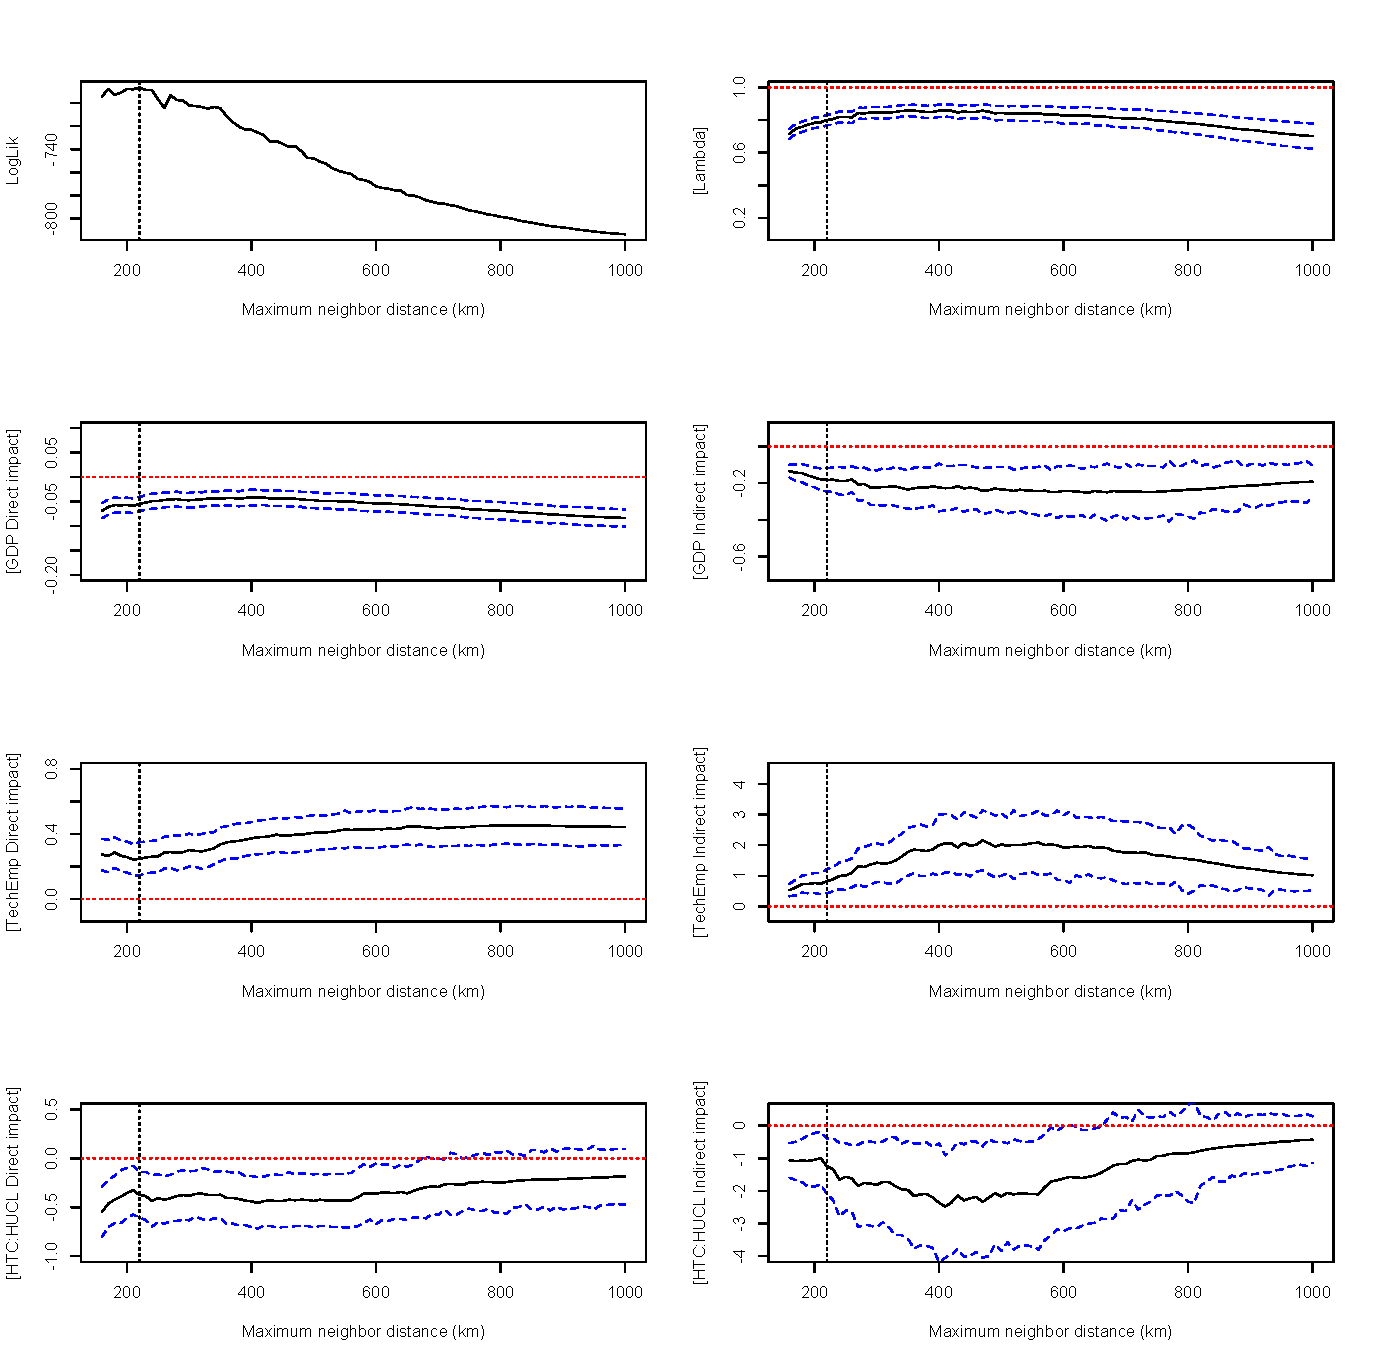
\includegraphics[width=.65\textwidth]{IMG/sp_Stability.pdf}
\end{figure}
\end{frame}
%---------------------------------------------------------------------
\section{Spatial filtering and semi-parametric models}
\begin{frame}{Spatial filtering and semi-parametric models}
\end{frame}
%---------------------------------------------------------------------
\begin{frame}{Spatial filtering and semi-parametric models}
\begin{itemize}
    \item Parametric methods are potentially not robust in a situation where the model suffers from a simultaneous presence of different sources of misspecification. \\Unaccounted nonlinear relationship among spatially correlated variables, spatially varying relationships (non-stationarity), uncontrolled common factors (spatial and time-related) and other instances of spatial heterogeneity can disrupt spatial dependencies or even manifest themselves as such. 
    \medskip
    \item Spatial filtering may be used to remove global and/or local spatial dependencies among geo-coded variables. 
    \medskip
    \item Spatial filtering does not rely on distributional assumptions and is fairly robust to model misspecification. 
\end{itemize}
\end{frame}
%---------------------------------------------------------------------
\begin{frame}{Spatial filtering and semi-parametric models}
\begin{itemize}
    \item Getis' nonparametric filtering can be used to eliminate spatial autocorrelation from observed data by ``spatial demeaning''. \\Based on $G_i(\tau)$ by Getis -- only applicable for positive spatial autocorrelation and positive support of the observed spatial variables.
    \bigskip
    \item Moran eigenvector map (MEM) filtering can be used to preserve some level of spatial properties within the model -- it is a semi-parametric method.
\end{itemize}
\end{frame}
%---------------------------------------------------------------------
\begin{frame}{Getis univariate filtering}
\begin{itemize}
    \item Approach based on $G_i(\tau)$ statistic by Getis: 
    $$
    G_i(\tau) = \frac{\sum_{j=1}^N c_{ij} \, y_j}{\sum_{j=1}^N y_j},
    \qquad ; \qquad
    E \left[G_i(\tau) \right] = \frac{c_i}{N}\,,
    $$
    where $c_i$ is the sum of elements of $i$-th row of $\bm{C}$ \\(note that $\bm{C}$ is used for filtering, not the $\bm{C}^{\ast} = \bm{C}+\bm{I}_N$).
    \bigskip
    \item Multiplicative transformation (filtering) of a spatial variable $y_i$: 
    \begin{equation*}
    \ddot{y}_i = \frac{E \left[G_i(\tau) \right]}{G_i(\tau)} \cdot y_i \>,
    \end{equation*}
    where $\ddot{y}_i$ is the spatially filtered value of $y_i$.
\end{itemize}
\end{frame}
%---------------------------------------------------------------------
\begin{frame}{Getis univariate filtering}
$$\ddot{y}_i = \frac{E \left[G_i(\tau) \right]}{G_i(\tau)} \cdot y_i \>,$$
\begin{itemize}
    \item Corrects for positive spatial autocorrelation in observed data by counterbalancing the clustering.
    \smallskip
    \item Filtering factor shrinks $y_i$ if the majority of observations $y_j$ within the $\tau$ distance of unit $i$ are above average. 
    \smallskip
    \item Similarly, $y_i$ is inflated if neighboring observations feature below-average values.
    \smallskip
    \item Simple and intuitive, yet positive support assumption can be a limitation. Also, the process of setting $\tau$ is arbitrary (robustness evaluation possible). 
    \item Univariate -- to estimate models using filtered data, such as $\bm{\ddot{y}} = 
  \alpha \bm{\iota} + \bm{\ddot{X} \beta} + \bm{\varepsilon} \, ,$ all variables have to be filtered individually.
\end{itemize}
\end{frame}
%---------------------------------------------------------------------
\begin{frame}{Moran's eigenvector map (MEM) filtering}
Econometric models are partitioned into two elements that are both employed within the spatial regression:
\medskip
\begin{itemize}
    \item  Exogenous regressors (say, macroeconomic indicators) 
    \smallskip
    \item Complementary spatial-filter variate (e.g. a MEM) describing spatial dependency that would otherwise affect model's residuals.
    \smallskip
    \item For MEM-based spatial filtering, all units need to be connected -- i.e. there has to be a ``path'' between any two regions, based on connections (edges) between neighboring units. Hence, for spatial filtering applications, $\tau$ value must not be lower than the longest edge of a minimum spanning tree of a graph based on $\bm{D}$ (where $d_{ij}$ are distances between units). Maximum limit on $\tau$ also applies (recall weak dependency assumptions).
\end{itemize}
\end{frame}
%---------------------------------------------------------------------
\begin{frame}{Semiparametric model with MEM-filter}
\begin{itemize}
    \item[1] Use $\bm{C}$ to construct a double-centered connectivity matrix $\bm{\Omega}$:
\begin{equation*}
\bm{\Omega} = (\bm{I}_N - \frac{1}{N}\,\bm{\iota}_N \bm{\iota}_N^{\prime})\, \bm{C} \, (\bm{I}_N - \frac{1}{N}\,\bm{\iota}_N \bm{\iota}_N^{\prime}) \,,
\end{equation*}
where $\bm{I}_N$ is the identity matrix and $\bm{\iota}_N$ is a column vector of ones. Double-centering standardizes $\bm{C}$ so that all rows and columns in $\bm{\Omega}$ add up to zero. $\bm{C}$ may be full rank (not guaranteed), $\bm{\Omega}$ is always rank deficient.
\medskip
\item[2] Calculate all distinct eigenvectors $\bm{v}_i$ and eigenvalues $\kappa_i$ for the double-centered matrix $\bm{\Omega}$ -- by solving the characteristic equation system  $(\bm{\Omega} - \kappa\, \bm{I}_{N}) \, \bm{v} = \bm{0} $. As $\bm{\Omega}$ is a real symmetric matrix, all distinct eigenvectors are orthogonal and linearly independent (given rank-deficiency of $\bm{\Omega}$, some eigenvalues and eigenvectors are duplicated). \\ \medskip 
MEM -- convenient subset of eigenvectors $\bm{v}$ -- can be used as a synthetic explanatory variable in semiparametric regression.
\end{itemize}
\end{frame}
%---------------------------------------------------------------------
\begin{frame}{Semiparametric model with MEM-filter}
\begin{itemize}
    \item[4] Semiparametric model is established using a misspecification paradigm and based on a regression model with spatially autocorrelated disturbances:
    \begin{equation*} 
    \begin{aligned}
    \bm{y} & = \bm{X\beta} + \bm{u} \,, \\
    \bm{u} & = \bm{E\gamma} + \bm{\varepsilon} \, ,
    \end{aligned}
    \end{equation*}
    where $\bm{u}$ are the spatially autocorrelated disturbances that may be decomposed into $\bm{\varepsilon}$ (white noise) and $\bm{E}$: a set of missing (unobservable) exogenous variables that follow common spatial dependency pattern ($\bm{C}$) and $\bm{\gamma}$ is a vector of parameters.
    \\ \medskip The $\bm{E\gamma}$ term is based on approximation and it is not directly comparable with the SEM parametric specification
\end{itemize}
\end{frame}
%---------------------------------------------------------------------
\begin{frame}{Semiparametric model with MEM-filter}
\begin{itemize}
    \item[5] Using a stepwise algorithm described next, the misspecification term $\bm{E}$ is approximated by MEM -- a convenient subset of Morans eigenvectors
\begin{equation*} 
\left\lbrace
\bm{v}_1, \dots , \bm{v}_{r} 
\right\rbrace 
\equiv 
\textnormal{evec}
\left(\bm{\Omega}\right) \, ,
\end{equation*}
where $r=\textnormal{rank}(\Omega)$ is the number of distinct eigenvectors of $\bm{\Omega}$. 
\\ \medskip 
We can approximate $\bm{E}$ by a parsimonious subset of eigenvectors $\bm{v}$ such that $\bm{M} = \left\lbrace \bm{v}_1, \dots , \bm{v}_{\ell} \right\rbrace$ where $\ell \leq r$. 
\\ \medskip 
Since spatial misspecification term $\bm{E}$ is correlated with $\bm{X}$ (at least potentially), the explicit inclusion of proxy element (MEM) $\bm{M}$ corrects for the bias in estimated coefficients $\hat{\bm{\beta}}$.
\end{itemize}
\end{frame}
%---------------------------------------------------------------------
\begin{frame}{Semiparametric model with MEM-filter}
\begin{itemize}
    \item[6] After substitution of $\bm{E}$ by $\bm{M}$, we get
\begin{equation*}
\bm{y} = \bm{X \beta } + \bm{M \gamma} + \bm{\varepsilon} \, ,
\end{equation*}
where $\bm{y}$ is decomposed into a systematic component (featuring $\bm{X}$), stochastic spatial component and white-noise residuals. 
\\ \medskip 
For conveniently specified $\bm{M}$, the stochastic spatial term $\bm{M \hat{\gamma}}$ removes a significant portion of the mean squared error (MSE) term, attributable to spatial autocorrelation 
\\ \medskip 
Hence, $\bm{M \hat{\gamma}}$ is often referred to as spatial filter. 
\\ \medskip 
Filtering is fairly robust to model specification errors when compared with fully parametric models.
\end{itemize}
\end{frame}
%---------------------------------------------------------------------
\begin{frame}{Semiparametric model with MEM-filter}
Stepwise algorithm for choosing $\bm{M}$:
\medskip
\begin{itemize}
    \item We choose $\bm{M}$ so that the residuals $\bm{\hat{\varepsilon}}$ become spatially random (independent with respect to the underlying spatial domain). 
    \smallskip
    \item We aim to find a parsimonious, i.e. smallest possible subset of eigenvectors $\bm{v}$, leading to spatial independence of $\bm{\hat{\varepsilon}}$.
    \smallskip
    \item Stepwise regression approach is often used.
    \smallskip
    \item Stepwise algorithm often based on a modified Moran's $I$ coefficient: Moran's $\textit{MC}$.
\end{itemize}
\end{frame}
%---------------------------------------------------------------------
\begin{frame}{Semiparametric model with MEM-filter}
Stepwise algorithm for choosing $\bm{M}\,$:
\medskip
\begin{itemize}
    \item $\textit{MC}_{\bm{v}_i} = \frac{N}{\bm{\iota}_N^{\prime} \, \bm{Z} \, \bm{\iota}_N } \, \bm{v}_i^{\prime} \bm{C} \bm{v}_i \, ,$\\ \smallskip
    where $\bm{Z}$ is a distance-based similarity matrix with $[z_{ij}] = 1 - (\tfrac{h_{ij}}{\textnormal{max}(h_{ij})})^2$. Individual $z_{ij}$ vary between zero for $h_{ij} = \textnormal{max}(h_{ij})$ and 1 for $h_{ij} = 0$.
    \smallskip
    \item First eigenvector is selected by maximizing $\textit{MC}_{\bm{v}_i}$. 
    \smallskip 
    \item Using such $\bm{v}_i$ as a starting eigenvector subset for $\bm{M}$, equation $\bm{y} = \bm{X \beta } + \bm{M \gamma} + \bm{\varepsilon}$ is estimated and residuals are evaluated for spatial autocorrelation (e.g. using Moran's $I$). 
    \smallskip
    \item If residuals are spatially dependent, new eigenvector is added to $\bm{M}$ using the same $\textit{MC}$ criterion, model is re-estimated and spatial autocorrelation in residuals is tested again. \smallskip 
    \item Eigenvectors are iteratively added to $\bm{M}$, until spatial autocorrelation in residuals $\bm{\hat{\varepsilon}}$ falls below a predetermined threshold (e.g. 5 \% significance level).
\end{itemize}
\end{frame}
%---------------------------------------------------------------------
\begin{frame}{Semiparametric model with MEM-filter}
$\bm{y} = \bm{X \beta } + \bm{M \gamma} + \bm{\varepsilon}$
\medskip
\begin{itemize}
    \item Eigenvectors in $\bm{M}$ are orthogonal and follow a strictly decreasing sequence.
    \smallskip
    \item Each eigenvector explains a specific proportion of variance in residuals of the model -- the largest proportion of variance is explained by the first eigenvector selected into $\bm{M}$, the second largest amount of variance is explained by the second eigenvector, etc. 
    \smallskip
    \item This leads to identical $\bm{M}$ matrices, obtained through forward and backward stepwise selection methods. 
    \smallskip
    \item Convenient linear combination of the above eigenvectors (i.e. $\bm{M\hat{\gamma}}$) is our spatial filter. 
    \smallskip
    \item Often, we only take into account positive spatial autocorrelation: only $\bm{v}_i$ associated with positive $\kappa_i$ are considered.
\end{itemize}
\end{frame}
%---------------------------------------------------------------------
\begin{frame}{Semiparametric model with MEM-filter}
$\bm{y} = \bm{X \beta } + \bm{M \gamma} + \bm{\varepsilon}$\\
\medskip
Individual $\bm{v}$ elements of $\bm{M}$ bear the following interpretation:\\
\bigskip
\begin{itemize}
    \item  MEMs -- spaces spanned by single or multiple $\bm{v}$ eigenvectors -- with associated ``large'' positive eigenvalues $\kappa_i$ represent global-scale spatial trends (say, landscape-wide dynamics in observed spatial data). 
    \medskip
    \item Eigenvectors with medium eigenvalues represent medium scale dynamics. 
    \medskip
    \item Eigenvectors with small positive eigenvalues would represent small scale dependencies (``local'' patchiness).   
\end{itemize}
\end{frame}
%---------------------------------------------------------------------
\begin{frame}{MEM - illustrative example}
\vspace{-0.3cm}
\begin{figure}
	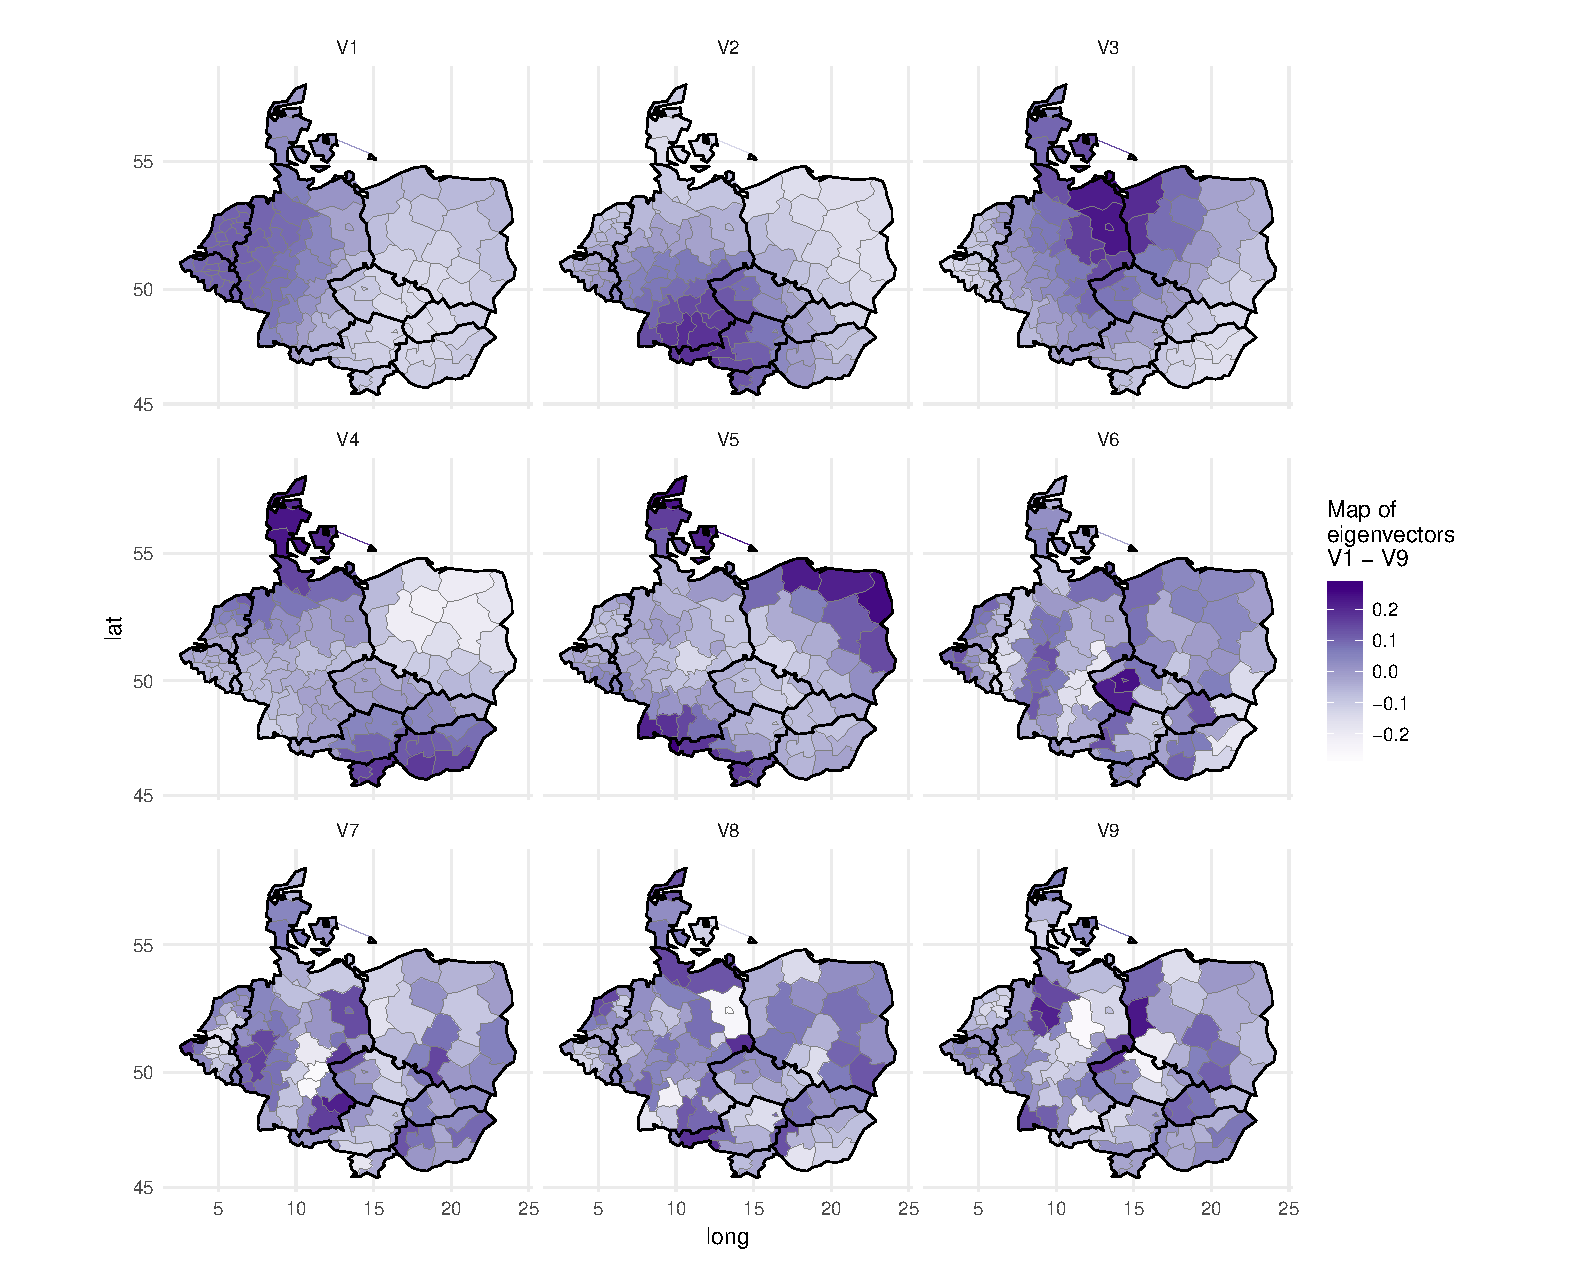
\includegraphics[width=.8\textwidth]{IMG/sp_Eigen.eps}
\end{figure}
\end{frame}
%---------------------------------------------------------------------
\section{Spatial panel models (parametric)}
\begin{frame}{Spatial panel models (parametric)}
\end{frame}
%---------------------------------------------------------------------
\begin{frame}{Spatial panel models}
For repeated geo-coded observations, spatial panel models depict interactions among variables across spatial units and over time:
\begin{equation*}
\begin{aligned}
  \bm{y}  &= 
  \lambda \left( \Ms{I}{T} \otimes \bm{W} \right) \bm{y} + \bm{X\beta} + \bm{u}\,, \\
  \bm{u} &= 
  \left( \Ms{\iota}{T} \otimes \Ms{I}{N} \right) \bm{\mu} + \bm{\varepsilon}\,, \\
  \bm{\varepsilon} &= \rho
  \left( \Ms{I}{T} \otimes \bm{W} \right) \bm{\varepsilon} + \bm{\upsilon}\,,
\end{aligned}
\end{equation*}
\small{where $\bm{y}$ is a $NT \!\times \!1$ column vector of dependent variable observations ($i = 1, 2, \dots, N$, $t=1,2, \dots, T$ and $i$ is the ``fast'' index). $\bm{W}$ is a spatial weights matrix and $\bm{X}$ is a $(NT \!\times \!k)$ matrix of exogenous regressors. Elements $\Ms{I}{T}$ and $\Ms{I}{N}$ are identity matrices and $\Ms{\iota}{T}$ is a  $(T \! \times \!1)$ vector of ones. Operator $\otimes$ is the Kronecker product. Elements of vector $\bm{\beta}$ as well as $\lambda$ and $\rho$ are parameters of the model. The disturbance vector $\bm{u}$ ($NT \!\times \!1$) is a sum of two terms: the unobserved individual effects $\bm{\mu}$ and spatially autocorrelated innovations $\bm{\varepsilon}$. The $(N \!\times \!1)$ vector $\bm{\mu}$ holds time-invariant and spatially uncorrelated individual effects. Innovations $\bm{\varepsilon}$ are spatially autocorrelated with a spatial error autoregressive parameter $\rho$ where $|\rho| < 1$. $\bm{\upsilon}$ is a vector of spatially independent innovations: $\upsilon_{it} \sim \textit{IID} \left( 0,\sigma_{\upsilon}^2 \right)$.}
\end{frame}
%---------------------------------------------------------------------
\begin{frame}{Spatial panel models}
\begin{equation*}
\begin{aligned}
  \bm{y}  &= 
  \lambda \left( \Ms{I}{T} \otimes \bm{W} \right) \bm{y} + \bm{X\beta} + \bm{u}\,, \\
  \bm{u} &= 
  \left( \Ms{\iota}{T} \otimes \Ms{I}{N} \right) \bm{\mu} + \bm{\varepsilon}\,, \\
  \bm{\varepsilon} &= \rho
  \left( \Ms{I}{T} \otimes \bm{W} \right) \bm{\varepsilon} + \bm{\upsilon}\,,
\end{aligned}
\end{equation*}
\begin{itemize}
    \item Spatial dependency  tests (Moran's $I$) for panel data are available.
    \smallskip
    \item By analogy to the GNS model (for CS data), the above specification is simplified (restricted) before estimation.
    \smallskip
    \item Generally, $\bm{\beta}$ parameters do not constitute marginal effects -- direct/indirect effects have to be calculated (using the same general approach as for CS data).
    \smallskip
    \item With ``random effects'' (RE) models, we assume that unobserved individual effects $\bm{\mu}$ are not correlated to other regressors of the model. 
    \smallskip
    \item For ``fixed effects'' (FE) models, some level of correlation between individual effects and other regressors is acceptable.
\end{itemize}
\end{frame}
%---------------------------------------------------------------------
\begin{frame}{Spatial panel models}
We shall briefly discuss three types of spatial panel models:
\bigskip
\begin{itemize}
    \item Fixed effects spatial lag model
    \medskip
    \item Fixed effects spatial error model
    \medskip
    \item Random effects spatial lag model
\end{itemize}
\end{frame}
%---------------------------------------------------------------------
\begin{frame}{Fixed effects spatial lag model}
\begin{itemize}
    \item FE spatial lag model that does not feature spatial autocorrelation in the error term can be written as 
\begin{equation*}
  \bm{y}  = 
  \lambda \left( \Ms{I}{T} \otimes \bm{W} \right) \bm{y} + 
  \left( \Ms{\iota}{T} \otimes \Ms{I}{N} \right) \bm{\mu} + 
  \bm{X \beta} + \bm{\upsilon} \,,
\end{equation*}
where $\bm{\upsilon}$ is a vector of spatially independent and normally distributed innovations.
\medskip
\item First step in FE spatial lag model estimation: eliminating the individual effects: 
\begin{equation*}
  \ddot{\bm{y}}  = 
  \lambda \left( \Ms{I}{T} \otimes \bm{W} \right) \ddot{\bm{y}} + 
  \ddot{\bm{X}} \bm{\beta} + \ddot{\bm{\upsilon}} \,,
\end{equation*}
where $\ddot{y}_{it}=y_{it}-\bar{y}_i$, etc.
\medskip
\item As individual effects are time-invariant, $\ddot{\mu}_{i}=\mu_{i}-\bar{\mu}_i=0$ \\and $\bm{\mu}$ disappears from equation.
\end{itemize}
\end{frame}
%---------------------------------------------------------------------
\begin{frame}{Fixed effects spatial lag model}
$$
\bm{y}  = 
  \lambda \left( \Ms{I}{T} \otimes \bm{W} \right) \bm{y} + 
  \left( \Ms{\iota}{T} \otimes \Ms{I}{N} \right) \bm{\mu} + 
  \bm{X \beta} + \bm{\upsilon}
$$
\begin{itemize}
    \item FE spatial lag model is estimated by MLE method. For detailed description, see \textcolor{blue}{\underline{\href{https://www.jstatsoft.org/article/view/v047i01}{Milo, Piras (2012)}}}
    \medskip
    \item Direct/indirect/total effects and their statistical significance is calculated (bootstrapped standard errors) -- see Milo, Piras (2012).
    \medskip
    \item From estimated FE model, we can calculate individual effects:
\begin{equation*}
\hat{\mu}_i =
\frac{1}{T} \sum_{t=1}^T \left[ y_{it} - \hat{\lambda} \left( \sum_{j=1}^N \! w_{ij} y_{jt} \right)
- \bm{x}_{it} \bm{\hat{\beta}} \right] \,.
\end{equation*}
However, for short panels $(N \gg T)$, enough observations for reliable $\mu_i$ estimation often do not accumulate.
\end{itemize}
\end{frame}
%---------------------------------------------------------------------
\begin{frame}{Fixed effects spatial error model}
\begin{itemize}
    \item Spatial lag is absent in the FE spatial error model:
    \begin{equation*}
    \begin{aligned}
      \bm{y}  &= 
      \left( \Ms{\iota}{T} \otimes \Ms{I}{N} \right) \bm{\mu} + \bm{X\beta} + \bm{\varepsilon}\,, \\
      \bm{\varepsilon} &= \rho
      \left( \Ms{I}{T} \otimes \bm{W} \right) \bm{\varepsilon} + \bm{\upsilon}\,.
    \end{aligned}
    \end{equation*}
    \item Model is estimated by MLE (time-demeaning is used).
    \smallskip
    \item Coefficients $\bm{\beta}$ are the marginal effects here
    \smallskip
    \item Individual effects can be retrieved from the estimated model as 
\begin{equation*} 
\hat{\mu}_i =
\frac{1}{T} \sum_{t=1}^T \left( y_{it} - \bm{x}_{it} \bm{\hat{\beta}} \right),
\end{equation*}
and reliability issues for short panels $(N \gg T)$ apply.
\end{itemize}
\end{frame}
%---------------------------------------------------------------------
\begin{frame}{Random effects spatial lag model}
\begin{itemize}
    \item Individual effects can be viewed as random and independent of regressors -- random effect (RE) model and RE estimator provide efficient estimates. RE properties of $\bm{\mu}$: \\$\mu_i \sim \textit{IID} \left( 0,\sigma_{\mu}^2 \right)$; normality is often assumed.
    \medskip
    \item Under RE assumptions, GNS panel model can be re-written as:
    \begin{equation*} 
     \begin{aligned}
      \bm{y}  &= 
      \lambda \left( \Ms{I}{T} \otimes \bm{W} \right) \bm{y} + \bm{X\beta} + \bm{u}\,, \\
      \bm{u} &= 
      \left( \Ms{\iota}{T} \otimes \Ms{I}{N} \right) \bm{\mu} + 
      \left( \Ms{I}{T} \otimes \Ms{B}{N}^{-1} \right) \bm{\upsilon}
     \end{aligned}
    \end{equation*}
    where $\Ms{B}{N}= \left( \Ms{I}{N} - \rho \bm{W} \right)$ and error variance may be outlined as
    \begin{equation*}
  \textnormal{var} \left( \bm{u} \right) = \bm{\Omega}_{\bm{u}} =
  \sigma_{\bm{\mu}}^2 \left( \Ms{\iota}{T} \Ms{\iota}{T}^\prime \otimes \Ms{I}{N} \right) 
  + \sigma_{\bm{\upsilon}}^2 \left[ \Ms{I}{T} \otimes \left( \Ms{B}{N}^\prime \Ms{B}{N} \right)^{-1} \right].
\end{equation*}
\end{itemize}
\end{frame}
%---------------------------------------------------------------------
\begin{frame}{Random effects spatial lag model}
    \begin{equation*} 
     \begin{aligned}
      \bm{y}  &= 
      \lambda \left( \Ms{I}{T} \otimes \bm{W} \right) \bm{y} + \bm{X\beta} + \bm{u}\,, \\
      \bm{u} &= 
      \left( \Ms{\iota}{T} \otimes \Ms{I}{N} \right) \bm{\mu} + 
      \left( \Ms{I}{T} \otimes \Ms{B}{N}^{-1} \right) \bm{\upsilon}
     \end{aligned}
    \end{equation*}
\begin{itemize}
    \item Model is estimated by MLE (iterative estimation involving concentrated $LL$ functions), see Milo, Piras (2012).
    \medskip
    \item Direct/indirect/total effects can be calculated.
    \medskip
    \item RE vs. FE: Generalized Hausman test can be applied: 
    \begin{equation*} 
    H = NT \left( \bm{\hat{\theta}}_{RE} - \bm{\hat{\theta}}_{FE} \right)^{\prime}
    \! \left( \bm{\hat{\Sigma}}_{RE} - \bm{\hat{\Sigma}}_{FE} \right)^{-1}
    \! \left( \bm{\hat{\theta}}_{RE} - \bm{\hat{\theta}}_{FE} \right)
    \,\,\, \underset{H_0}{\sim} \,\,\, \chi_k^2 \,\,,
\end{equation*}
where $\bm{\hat{\theta}}_{RE}$ and $\bm{\hat{\theta}}_{FE}$ are the RE and FE-based estimates, $\bm{\hat{\Sigma}}_{RE}$ and $\bm{\hat{\Sigma}}_{FE}$ are corresponding variance-covariance matrices. Under $H_0$ (RE assumptions hold), the test statistic is asymptotically $\chi^2$-distributed with $k$ d.f. ($k$ is the number of regressors).
\end{itemize}
\end{frame}
%---------------------------------------------------------------------
\begin{frame}{Spatial analysis and regression models in R}
\begin{itemize}
	\item \{spdep\} 
	\item \{splm\}
	\item \{sf\}, \{sp\}, \{ggplot2\}
	\item \textcolor{blue}{\underline{\href{https://cran.r-project.org/web/views/Spatial.html}{https://cran.r-project.org/web/views/Spatial.html}}}
\end{itemize}
 \begin{figure}
 	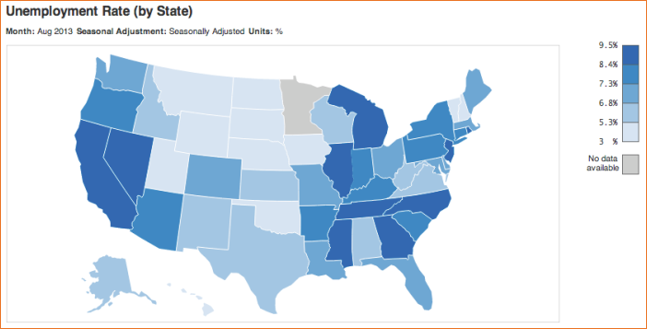
\includegraphics[width=.7\textwidth]{IMG/sp_unemp.PNG}
 \end{figure}
\end{frame}
%---------------------------------------------------------------------
\end{document}